\chapter{Tính năng AI của hệ thống}
\textit{Chương này trình bày các tính năng AI cốt lõi của hệ thống, tập trung vào hai năng lực chính là đánh giá kỹ năng Speaking và đánh giá kỹ năng Writing. Đối với Speaking, nhóm đã hiện thực một nền tảng chuyên biệt mang tên \textbf{Lingriser} nhằm tổ chức lộ trình luyện nói, hội thoại với AI và phối hợp cùng giáo viên/mentor. Đối với Writing, hệ thống tập trung vào định hướng chấm điểm và phân tích bài viết để nâng cao hiệu quả học tập cho người dùng.}


\section{Tính năng AI cho Speaking - Giới thiệu LingriserSpeaking}
Lingriser được sinh ra để hỗ trợ tính năng AI cho speaking cho trang web. Lingriser là nền tảng luyện nói tiếng Anh được xây dựng cho học sinh Việt Nam với mục tiêu hình thành một môi trường luyện tập có cấu trúc sư phạm.

Thay vì tách rời giữa học trên lớp, tự học và phản hồi cá nhân hóa, Lingriser liên kết ba thành phần này trong một chu trình thống nhất gồm: học trực tiếp với giáo viên vào đầu tuần, luyện nói cùng AI trong tuần và tham gia buổi gọi video với mentor vào cuối tuần. Cách tổ chức này giúp AI đóng vai trò như một lớp hỗ trợ trung gian, duy trì cường độ luyện tập và chuẩn bị cho người học trước khi bước vào tương tác thực tế.

Điểm khác biệt quan trọng của hệ thống là học sinh không dừng lại ở việc luyện nói với AI, mà còn có thể chủ động \textit{book} lịch video call với giáo viên hoặc mentor bản ngữ để thực hành giao tiếp trong môi trường đồng bộ. Nhờ đó, kết quả của giai đoạn tự luyện không bị tách rời mà được nối tiếp trực tiếp sang tương tác với người thật.

Bên cạnh đó, nền tảng cũng cho phép phụ huynh theo dõi tình hình học tập của con thông qua dashboard riêng. Cơ chế này giúp phụ huynh quan sát tiến độ luyện nói, mức độ tham gia và các tín hiệu cải thiện theo thời gian, thay vì chỉ nhận các thông tin rời rạc sau từng buổi học.

\subsection{Cấu trúc học tập và các vai trò người dùng}

Mỗi khóa học trên Lingriser được tổ chức thành \textbf{8 module hằng tuần}. Trong mỗi module, ba hoạt động học tập được phân tầng theo ngày trong tuần, tạo thành một chu trình luyện tập khép kín:

\begin{table}[H]
\centering
\begin{tabular}{|l|l|p{7.5cm}|}
\hline
\textbf{Thời điểm} & \textbf{Hoạt động} & \textbf{Mô tả} \\ \hline
Thứ Hai & Học trực tiếp & Buổi học trên lớp do giáo viên người Việt giảng dạy; giáo viên đặt \textit{weekly focus} (mục tiêu luyện nói trọng tâm) cho cả tuần \\ \hline
Thứ Ba -- Thứ Sáu & Luyện AI & Học sinh tự luyện nói với đối tác hội thoại AI theo chủ đề và mục tiêu của giáo viên; hệ thống phiên âm, phản hồi và tổng hợp giọng nói \\ \hline
Thứ Bảy -- Chủ Nhật & Gọi video & Buổi 1-on-1 với mentor bản ngữ qua Google Meet; mentor nhận bản tóm tắt tiến trình luyện AI trước buổi gọi \\ \hline
\end{tabular}
\caption{Lịch trình hoạt động học tập hằng tuần trên Lingriser}
\end{table}

Nền tảng phục vụ năm vai trò người dùng với phạm vi truy cập và chức năng riêng biệt:

\begin{table}[H]
\centering
\begin{tabular}{|l|p{9.5cm}|}
\hline
\textbf{Vai trò} & \textbf{Phạm vi chức năng} \\ \hline
\texttt{student} & Dashboard cá nhân, luyện nói với AI, đặt lịch video call, theo dõi tiến trình theo module \\ \hline
\texttt{teacher} & Dạy lớp thứ Hai, đặt \textit{weekly focus} cho từng module để định hướng AI practice và mentor \\ \hline
\texttt{mentor} & Thực hiện buổi gọi video cuối tuần, xem \textit{mentor brief} tổng hợp từ kết quả luyện AI \\ \hline
\texttt{parent} & Theo dõi lịch học, mức độ tham gia luyện AI và chỉ báo tiến bộ hằng tuần của con \\ \hline
\texttt{admin} & Quản lý toàn bộ người dùng, khóa học, chương trình học và thống kê nền tảng \\ \hline
\end{tabular}
\caption{Các vai trò người dùng trên nền tảng Lingriser}
\end{table}

\begin{figure}[H]
    \centering
    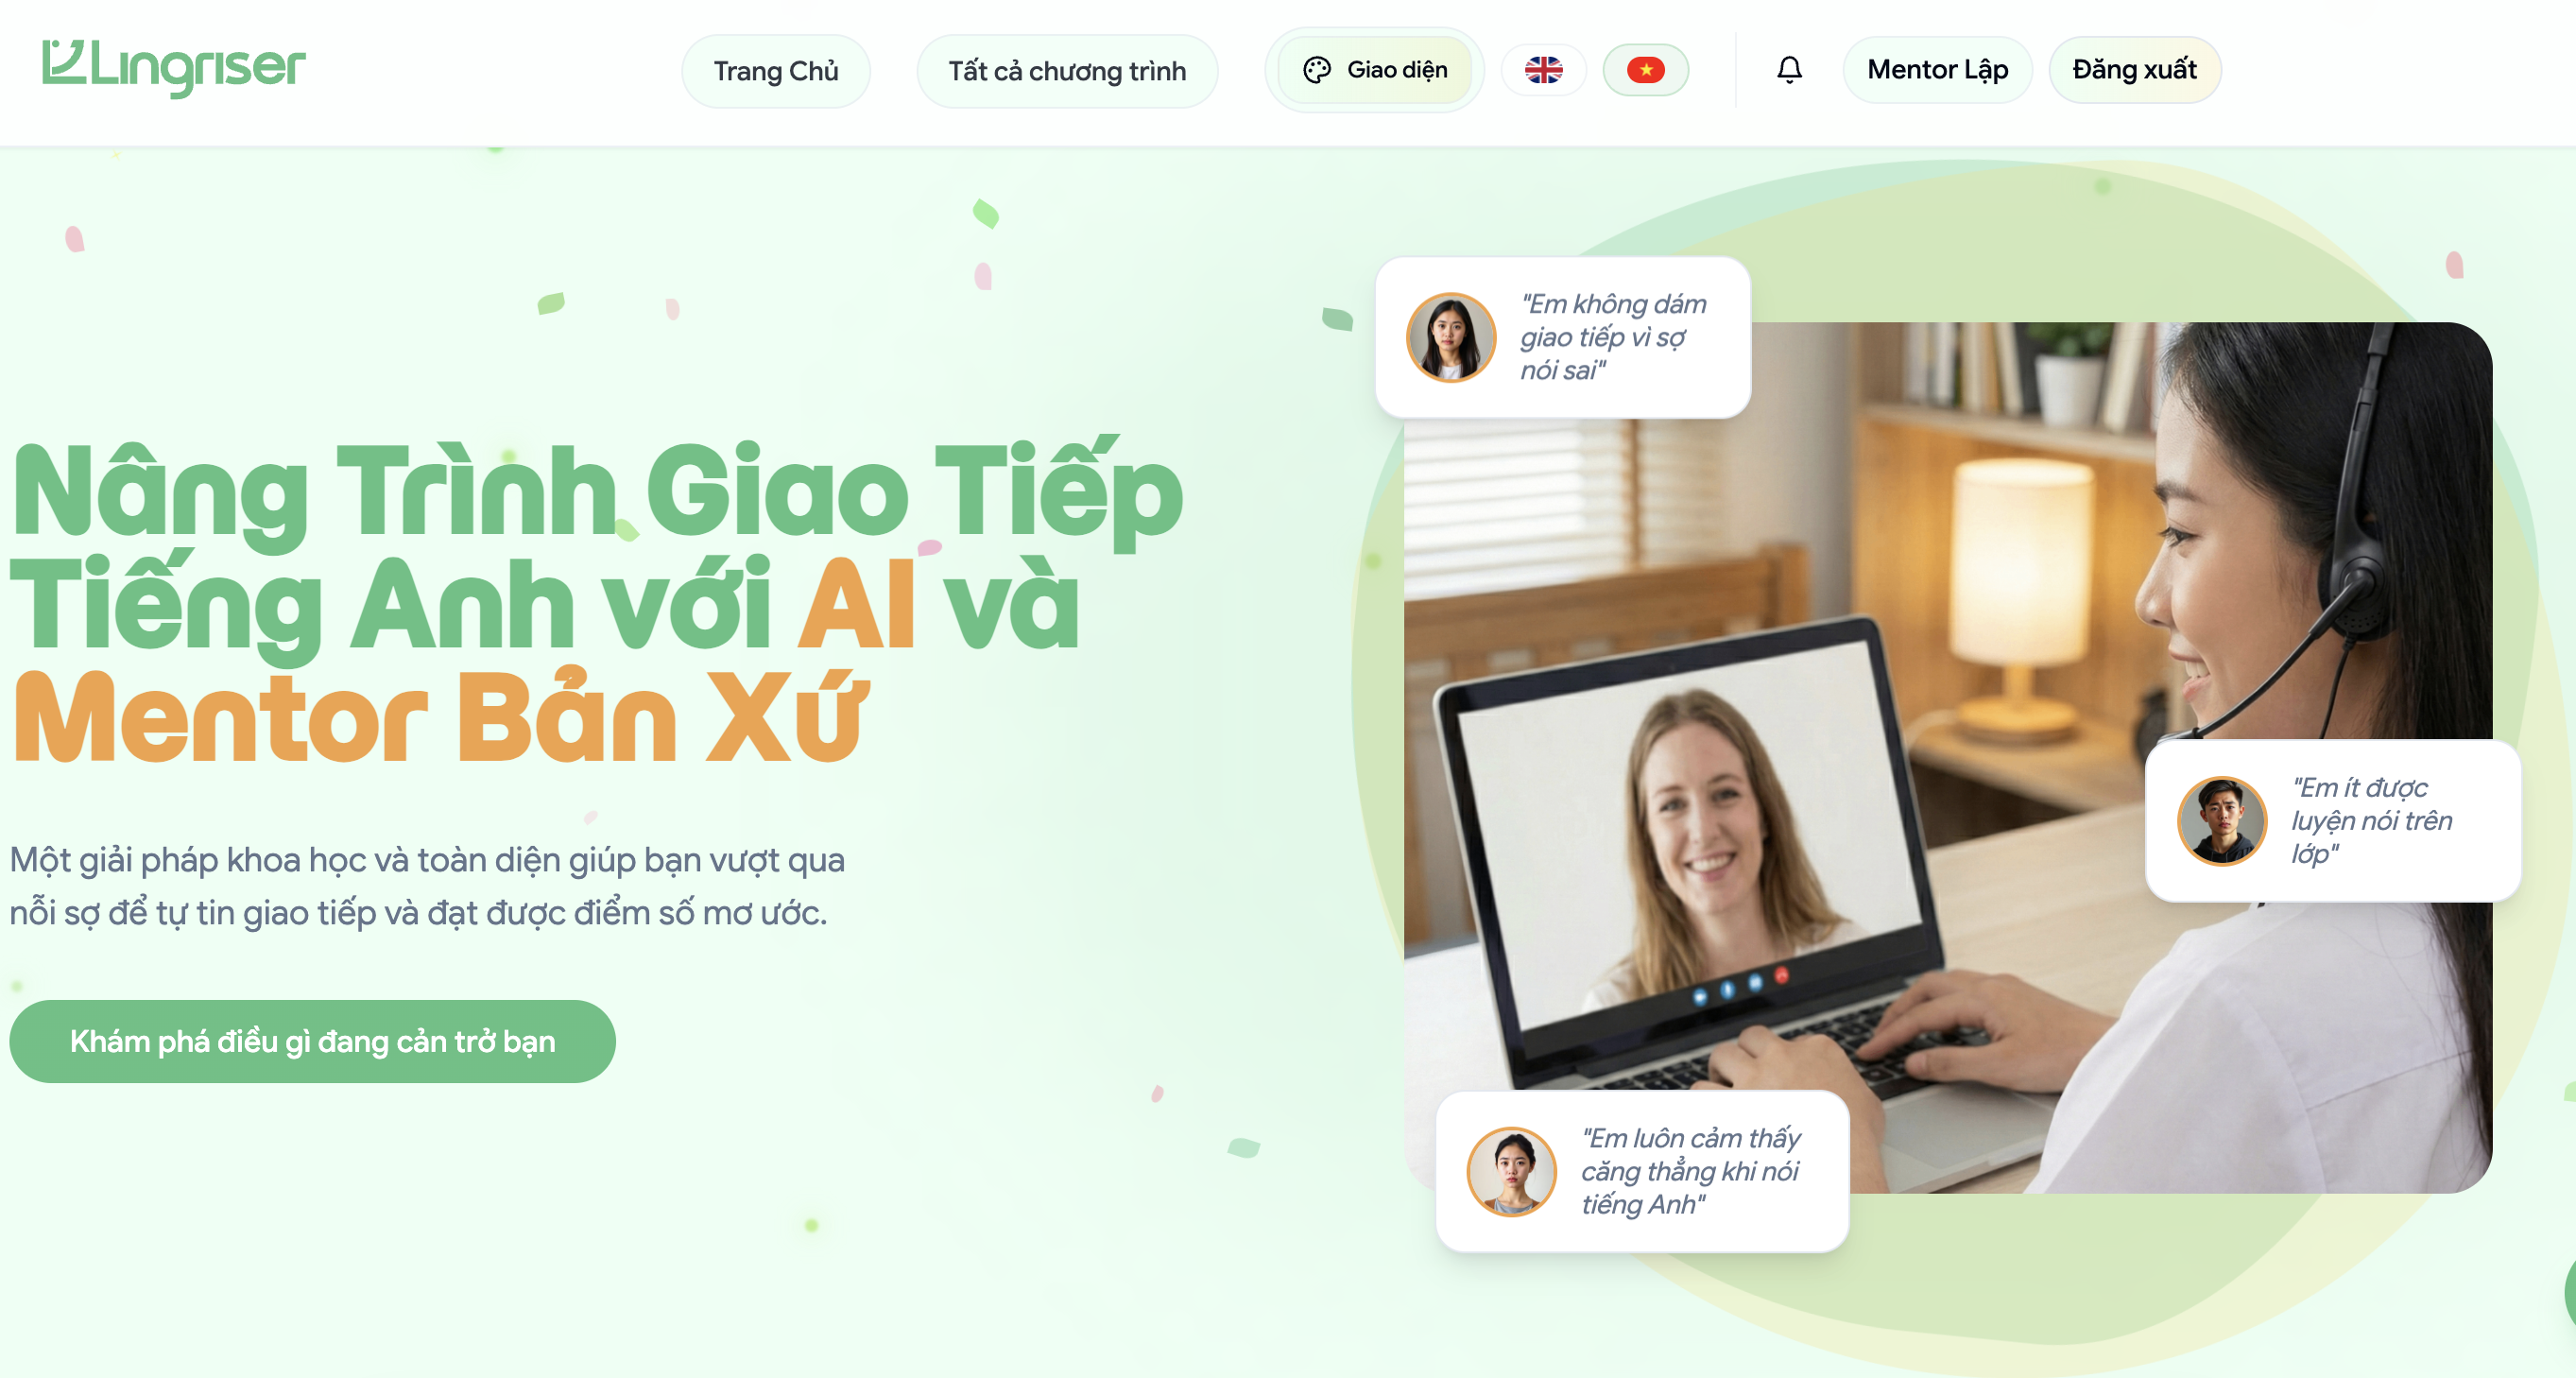
\includegraphics[width=0.92\linewidth]{graphics/lingriser/dashboard}
    \captionsetup{skip=5pt}
    \caption{Giao diện tổng quan của nền tảng Lingriser dành cho học sinh}
\end{figure}

Từ góc nhìn chức năng, mô-đun Speaking trong Lingriser được thiết kế xoay quanh ba mục tiêu chính. Thứ nhất, hệ thống tạo điều kiện để người học luyện phản xạ nói hằng ngày thông qua đối tác hội thoại AI. Thứ hai, AI được dùng để phiên âm, phản hồi và nhắc lại nội dung bằng giọng nói tổng hợp, qua đó tạo thành vòng lặp nghe -- nói -- tự điều chỉnh gần với trải nghiệm giao tiếp thật. Thứ ba, dữ liệu luyện tập được gắn với chương trình học theo tuần để giáo viên và mentor có thể theo dõi, định hướng và kế thừa kết quả của người học trong các buổi học tiếp theo.

\subsection{Mô hình học tập kết hợp AI và con người}
Điểm đặc trưng của Lingriser nằm ở việc AI không hoạt động độc lập mà được đặt trong một hệ sinh thái học tập kết hợp giữa nhà trường, giáo viên, mentor và phụ huynh. Mỗi khóa học được chia thành các module hằng tuần. Trong từng module, giáo viên có thể đặt ra \textit{weekly focus} -- tức mục tiêu luyện nói trọng tâm mà học sinh cần bám theo. Các mục tiêu này sau đó được chuyển xuống mô-đun AI practice để định hướng nội dung hội thoại, đồng thời được hiển thị cho mentor trước buổi gọi video cuối tuần. Nhờ đó, nội dung luyện nói với AI không bị rời rạc mà bám sát tiến trình học tập thực tế.

Ngoài lớp phối hợp giữa giáo viên và mentor, Lingriser còn hiện thực cơ chế liên kết giữa tài khoản phụ huynh và học sinh. Thông qua mối quan hệ này, phụ huynh có thể theo dõi tiến trình tham gia của con em mình, bao gồm lịch học, mức độ luyện AI và một số chỉ báo tiến bộ theo tuần. Việc đưa phụ huynh vào vòng theo dõi không trực tiếp làm thay đổi mô hình AI, nhưng làm tăng giá trị của dữ liệu do AI tạo ra: kết quả phiên âm, phản hồi sau buổi luyện và thống kê luyện tập không chỉ phục vụ người học mà còn trở thành cơ sở để gia đình đồng hành cùng quá trình rèn luyện Speaking.

\begin{figure}[H]
    \centering
    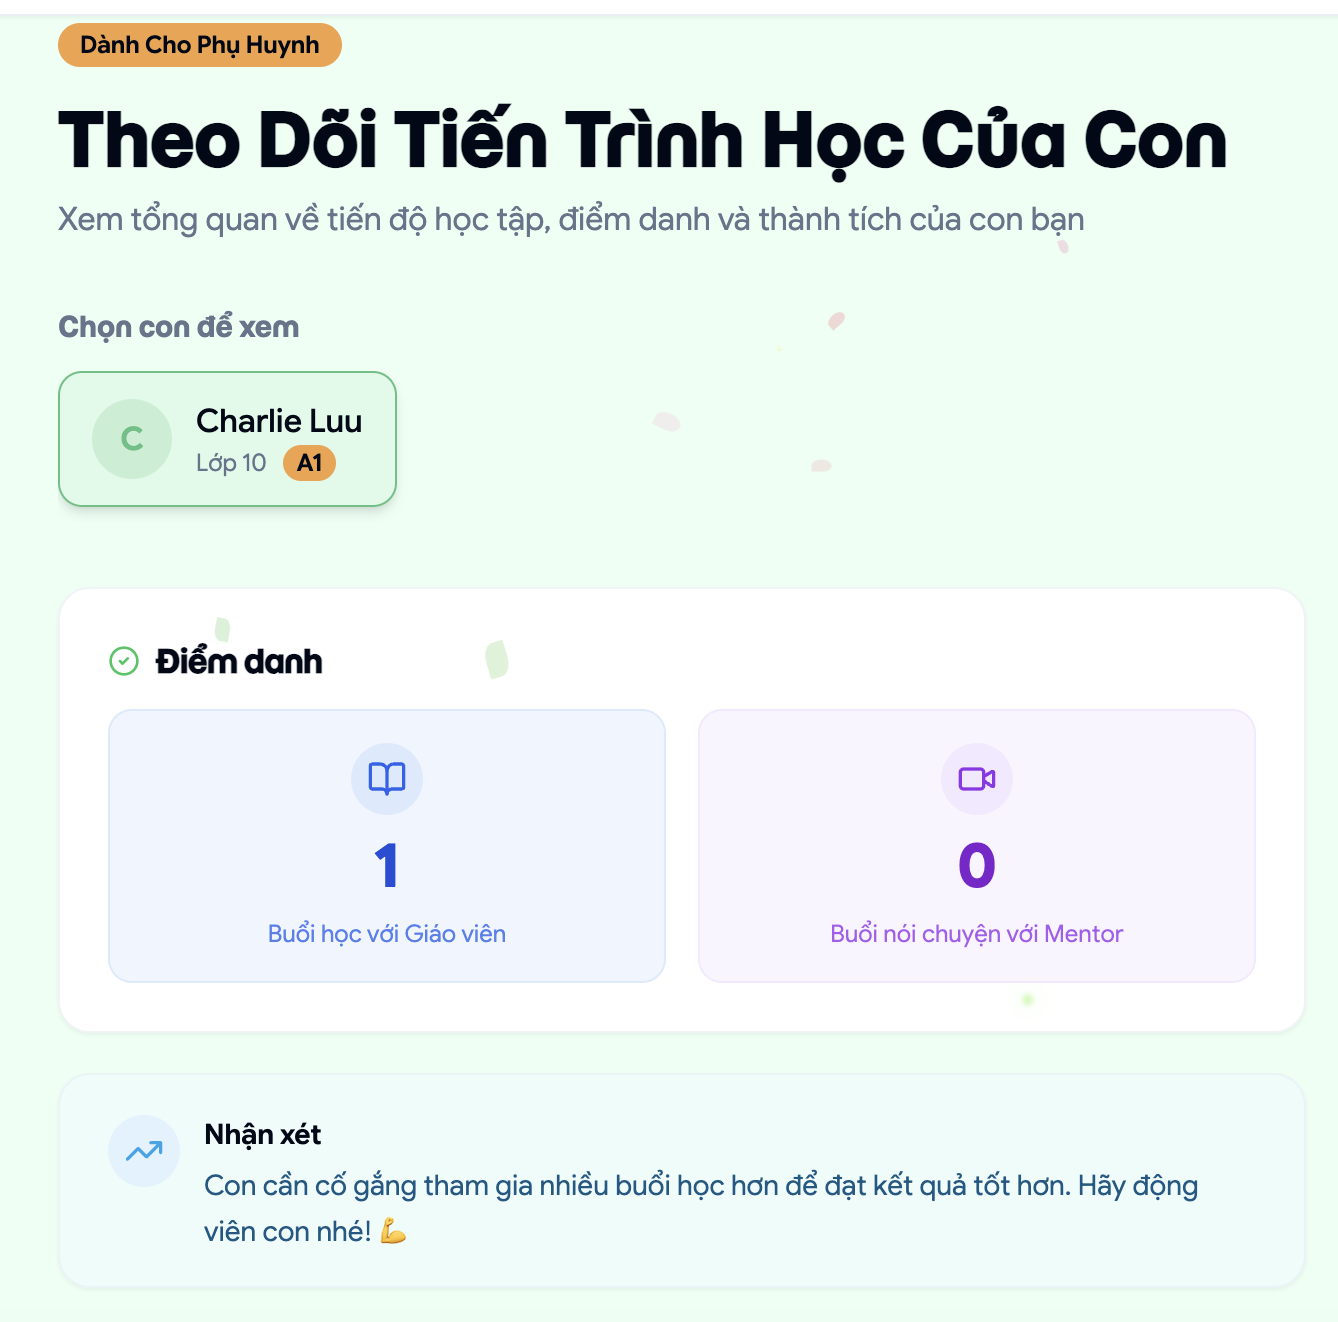
\includegraphics[width=0.88\linewidth]{graphics/lingriser/parents}
    \captionsetup{skip=5pt}
    \caption{Giao diện theo dõi tiến trình học sinh từ phía phụ huynh trên Lingriser}
\end{figure}

\begin{figure}[H]
    \centering
    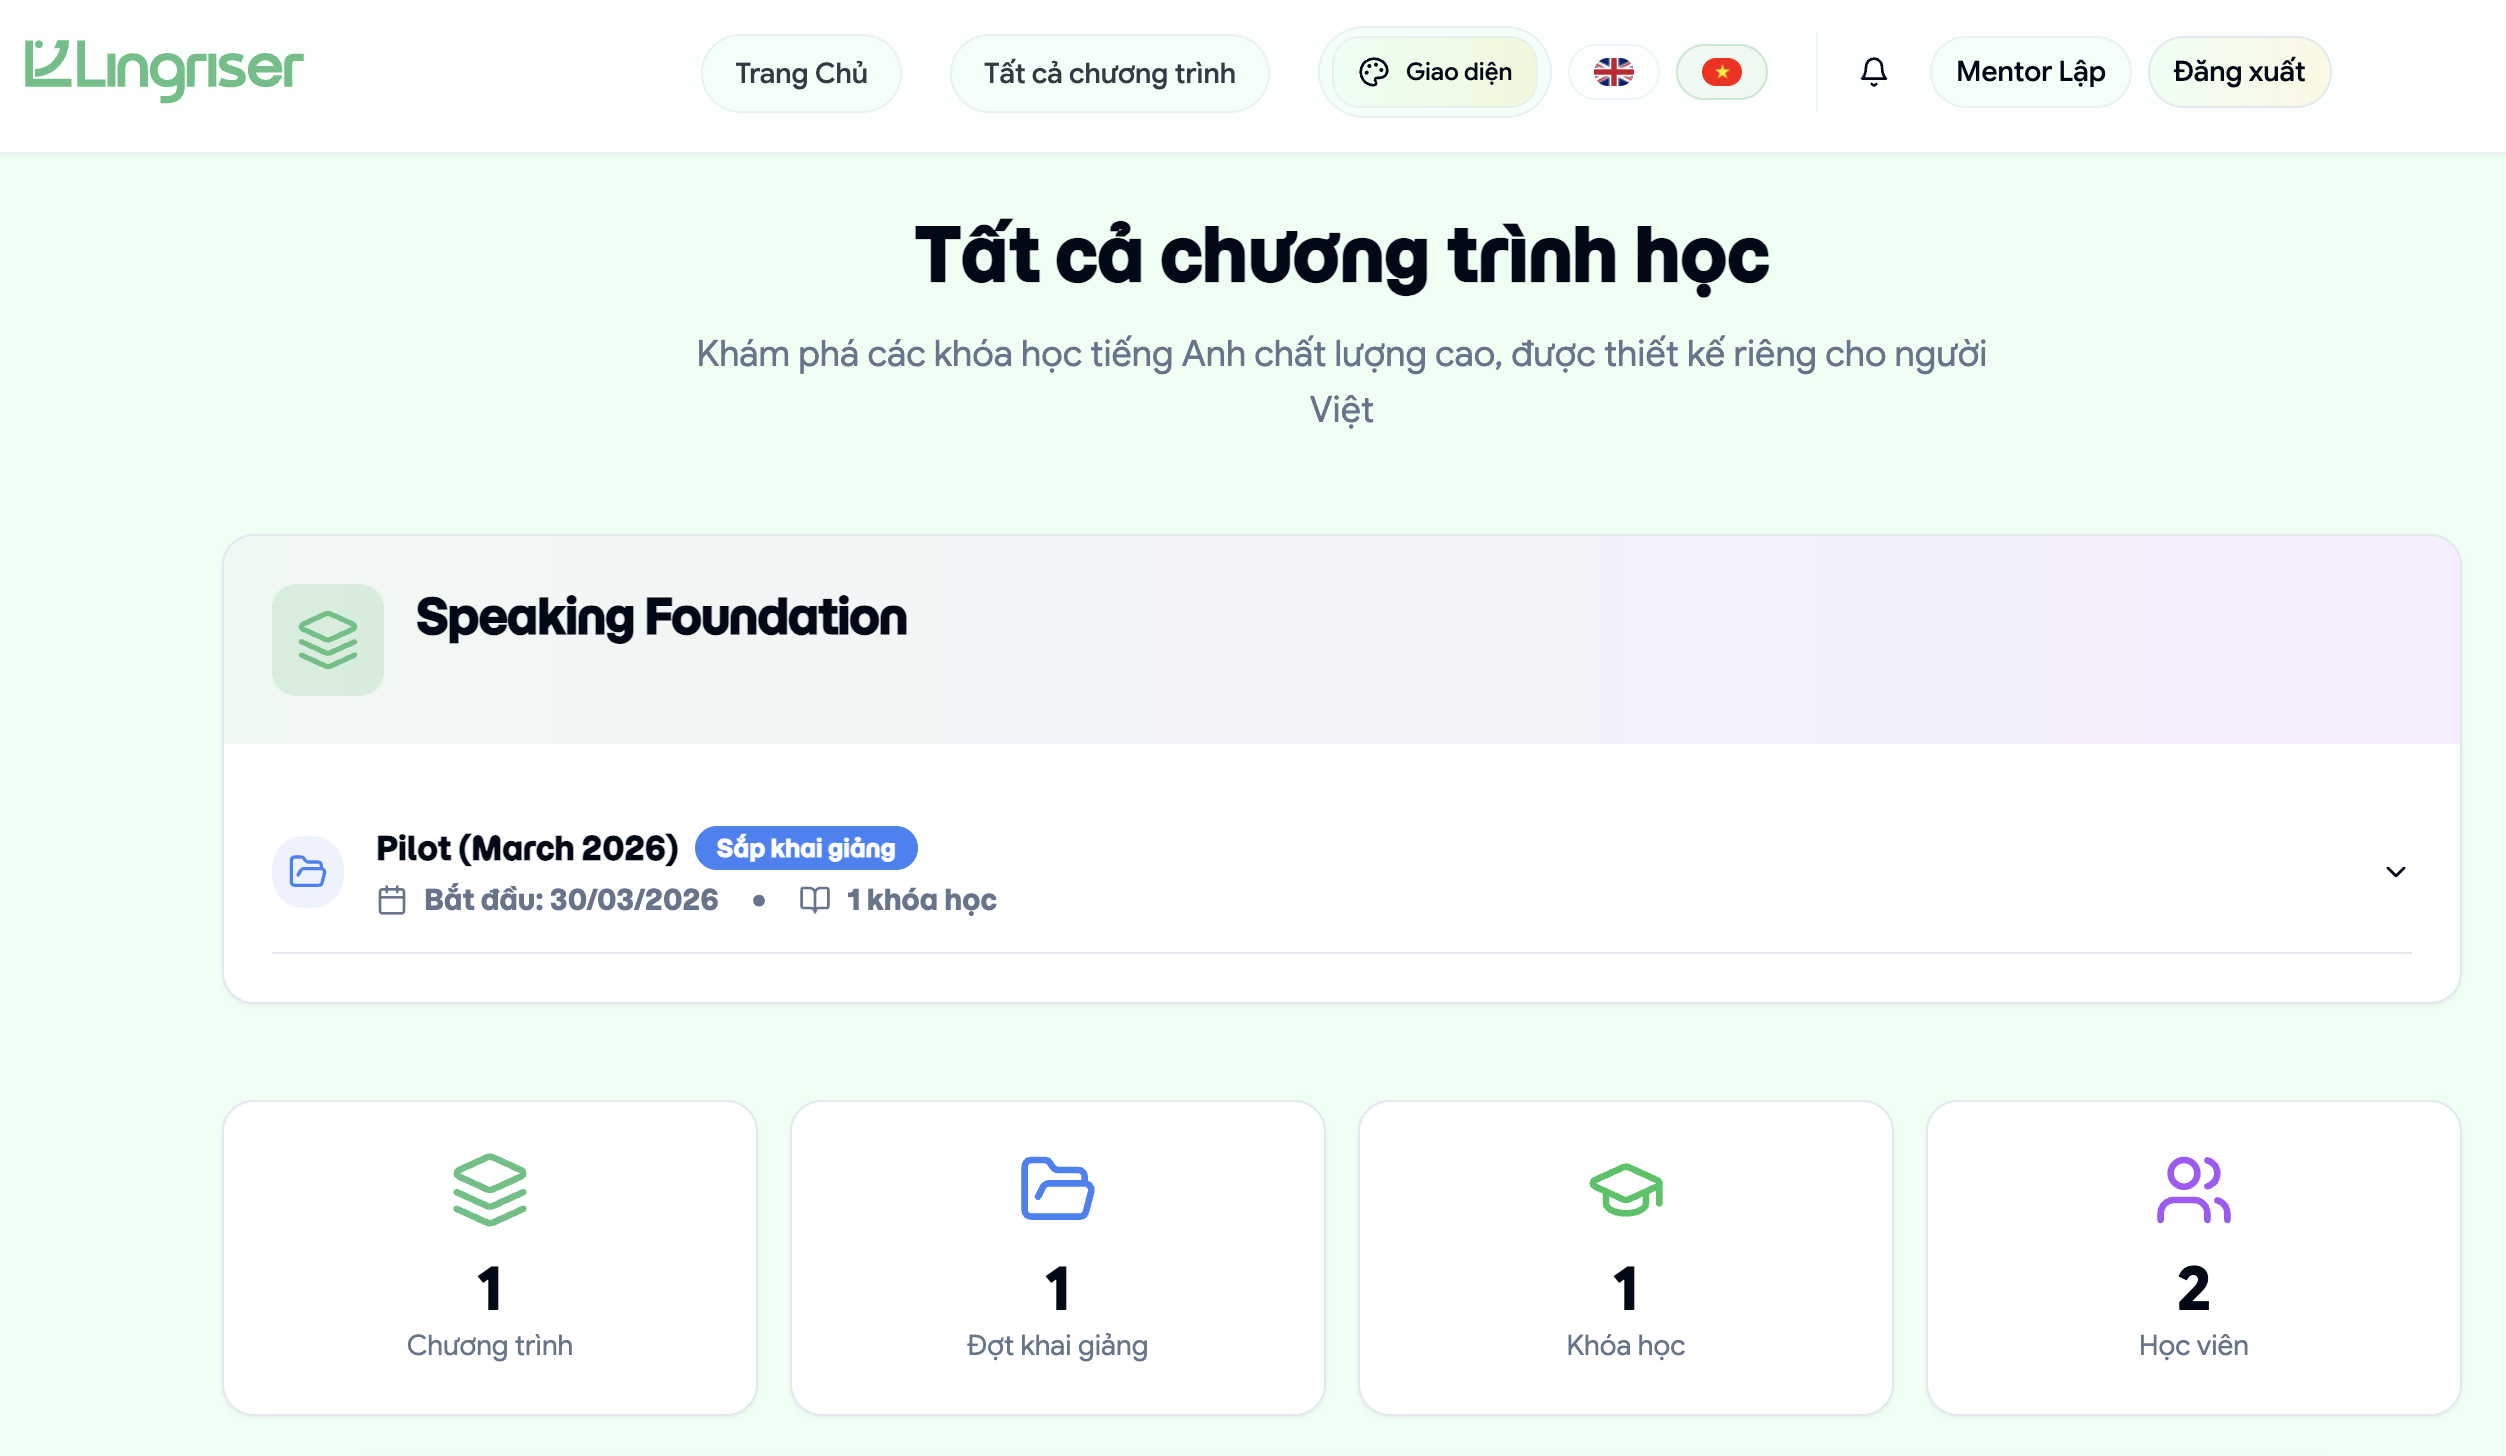
\includegraphics[width=0.9\linewidth]{graphics/lingriser/programs}
    \captionsetup{skip=5pt}
    \caption{Quản lý chương trình học và tiến trình theo module trong Lingriser}
\end{figure}

Cách tiếp cận này mang lại hai lợi ích quan trọng. Về mặt sư phạm, nó tạo ra sự liên tục giữa mục tiêu học tập, hoạt động luyện tập và đánh giá sau luyện tập. Về mặt hệ thống, nó cho phép AI cá nhân hóa phản hồi theo bối cảnh cụ thể của từng học sinh thay vì chỉ sinh câu trả lời tổng quát. Đây là một điểm khác biệt quan trọng giữa Lingriser và các ứng dụng luyện nói chỉ cung cấp hội thoại tự do không có định hướng.

\subsection{Các thành phần AI cốt lõi trong Lingriser}

Mô-đun AI Practice của Lingriser được hiện thực trong \texttt{AIPracticeService} (NestJS), giao tiếp trực tiếp với OpenAI API qua SDK chính thức. Có bốn endpoint API tương ứng với bốn tác vụ AI riêng biệt:

\begin{table}[H]
\centering
\begin{tabular}{|l|l|p{6cm}|}
\hline
\textbf{Method} & \textbf{Endpoint} & \textbf{Chức năng} \\ \hline
POST & \texttt{/api/ai-practice/chat} & Hội thoại GPT-4o-mini (non-streaming) \\ \hline
POST & \texttt{/api/ai-practice/transcribe} & Phiên âm audio Whisper-1 (multipart) \\ \hline
POST & \texttt{/api/ai-practice/tts} & Chuyển văn bản thành giọng nói MP3 \\ \hline
POST & \texttt{/api/ai-practice/feedback} & Sinh phân tích buổi luyện từ transcript \\ \hline
\end{tabular}
\caption{Các API endpoint của mô-đun AI Practice}
\end{table}

\begin{figure}[H]
    \centering
    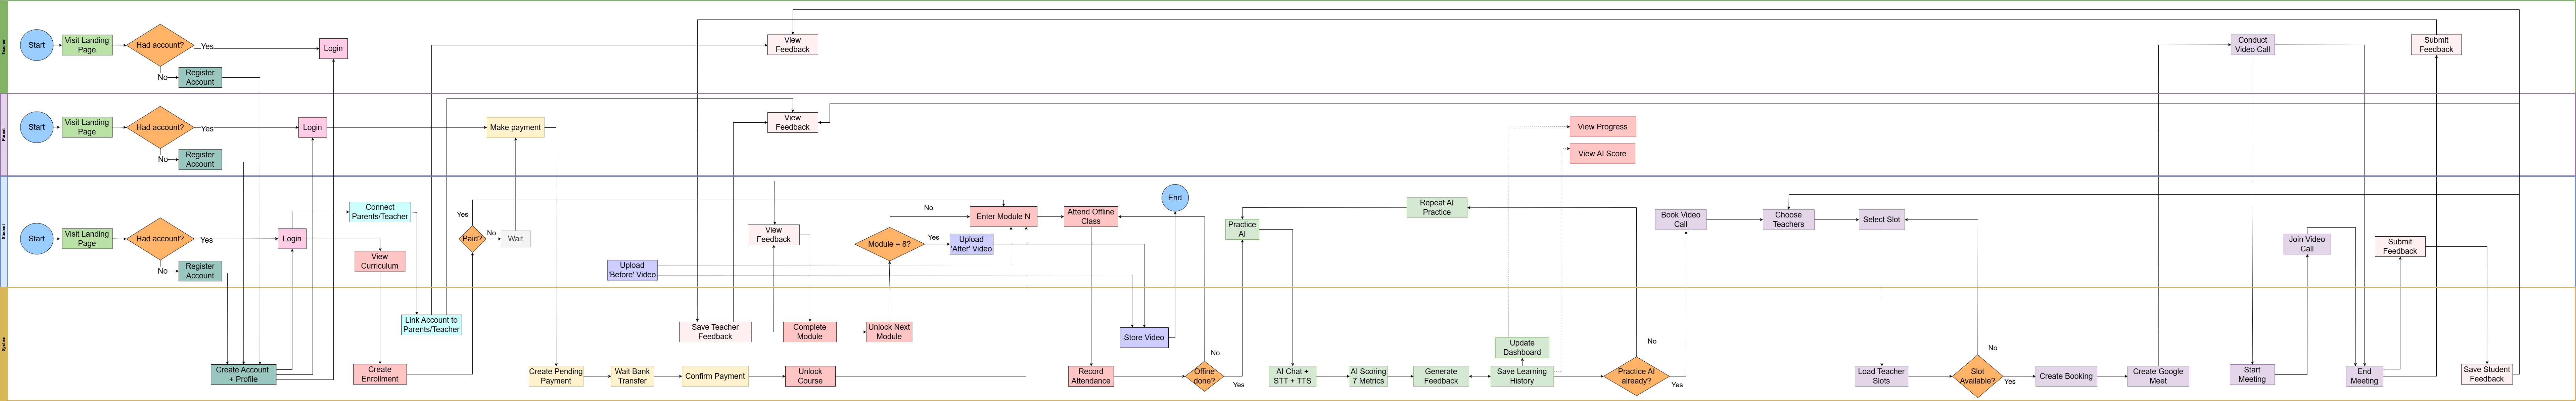
\includegraphics[width=\linewidth]{graphics/lingriser/system_architecture}
    \captionsetup{skip=5pt}
    \caption{Kiến trúc triển khai của Lingriser với mô-đun AI Practice}
\end{figure}

\subsubsection{System Prompt Engineering cho hội thoại}

Điểm kỹ thuật then chốt là hàm \texttt{buildSystemPrompt()} được gọi mỗi lần khởi tạo cuộc hội thoại. Hàm này tổng hợp ngữ cảnh từ ba nguồn thành một system prompt duy nhất truyền vào GPT-4o-mini:

\begin{enumerate}
    \item \textbf{Trình độ CEFR:} Mỗi level ánh xạ sang một bộ hướng dẫn ngôn ngữ cụ thể. Ví dụ, \texttt{beginner} → \textit{"Use simple vocabulary and short sentences. Avoid complex grammar."}, còn \texttt{advanced} → \textit{"Use rich vocabulary, complex grammar, and natural expressions like a native speaker."} Tham số \texttt{temperature = 0.8} và \texttt{max\_tokens = 500} được cố định để đảm bảo phản hồi đa dạng nhưng không quá dài.

    \item \textbf{Weekly Focus Goals:} Nếu mảng \texttt{speakingGoals[]} từ bảng \texttt{weekly\_focus} không rỗng, từng mục tiêu được nối thành một khối \texttt{WEEKLY SPEAKING GOALS} trong system prompt, kèm hướng dẫn để AI nhẹ nhàng dẫn dắt hội thoại về phía các mục tiêu đó. Đây là cơ chế kỹ thuật kết nối dữ liệu của giáo viên với hành vi của mô hình AI.

    \item \textbf{Quy tắc hội thoại nghiêm ngặt:} System prompt mã hóa bốn ràng buộc cứng: (a) bám sát chủ đề, tối đa một câu follow-up về chi tiết phụ rồi quay lại chủ đề chính; (b) không bình luận dài dòng, chỉ hỏi câu tiếp theo; (c) phản hồi tối đa 1--2 câu; (d) cuối mỗi lượt trả về 2--3 câu gợi ý theo định dạng JSON với key \texttt{suggestions} kẹp giữa hai marker cố định \texttt{---SUGGESTIONS---} và \texttt{---END---}. Frontend parse khối này để hiển thị gợi ý tách biệt với nội dung hội thoại chính.
\end{enumerate}

\subsubsection{Phiên âm Whisper và thuật toán Pause Detection}

Khi học sinh gửi audio, backend gọi Whisper-1 với cấu hình \texttt{response\_format: 'verbose\_json'} và \texttt{timestamp\_granularities: ['word']} để nhận timestamp cấp độ từng từ thay vì chỉ chuỗi văn bản. Whisper còn được truyền vào một prompt hướng dẫn phiên âm nguyên văn, không tự động sửa lỗi phát âm, không bổ sung từ thiếu — nhằm bảo toàn các lỗi thực tế của học sinh để phân tích.

Dữ liệu \texttt{words[]} từ Whisper sau đó được đưa vào thuật toán Pause Detection trong \texttt{generateFeedback()}:

\begin{enumerate}
    \item Với mỗi lượt nói của học sinh, duyệt qua danh sách từ theo thứ tự \texttt{start} timestamp.
    \item Tính khoảng cách giữa hai từ liên tiếp: $\text{gap} = w_i.\text{start} - w_{i-1}.\text{end}$.
    \item Nếu $\text{gap} > 0.5$ giây: tăng \texttt{pauseCount}, đánh dấu lượt đó vào \texttt{pauseTurns}, chèn marker \texttt{"uhmmm"} vào bản phiên âm để phản ánh khoảng ngừng thực tế.
    \item Kết quả lưu vào cột \texttt{pause\_detection JSONB} của bảng \texttt{ai\_feedback}, gồm các trường \texttt{has\_pause}, \texttt{pause\_count}, \texttt{pause\_turns[]} và \texttt{summary} mô tả bằng tiếng Việt.
\end{enumerate}

Ngoài pause detection, hệ thống còn tính \texttt{response\_duration} — thời gian phát biểu trung bình mỗi lượt — bằng cách đo khoảng cách từ \texttt{words[0].start} đến \texttt{words[last].end}. Nếu không có dữ liệu timestamp (chế độ chat text), hệ thống ước lượng theo tốc độ phát biểu trung bình 2,2 từ/giây. Toàn bộ analytics sau đó được gắn với bản ghi \texttt{learning\_history} tương ứng để phục vụ thống kê trên dashboard.

\subsubsection{Text-to-Speech và vòng lặp nghe--nói}

Phản hồi văn bản từ GPT-4o-mini được chuyển thành giọng nói qua \texttt{gpt-4o-mini-tts} với giọng \texttt{alloy}, định dạng MP3. Backend trả buffer MP3 trực tiếp trong response body (\texttt{Content-Type: audio/mpeg}); frontend nhận và phát âm thanh ngay lập tức, tạo vòng lặp nghe--nói liên tục mà không cần tải file về.

\subsection{Luồng luyện Speaking trên nền tảng}
Quy trình luyện nói trong Lingriser được tổ chức thành nhiều bước rõ ràng. Trước tiên, học sinh truy cập giao diện luyện tập từ dashboard cá nhân. Hệ thống tải thông tin module hiện tại, các mục tiêu \textit{weekly focus} và dữ liệu tiến độ liên quan. Tiếp theo, người dùng bắt đầu phiên luyện nói bằng giao diện chat hoặc ghi âm. Trong quá trình này, AI duy trì ngữ cảnh hội thoại để đặt câu hỏi nối tiếp phù hợp thay vì phản hồi rời rạc từng câu riêng lẻ.

Sau khi học sinh gửi câu trả lời bằng giọng nói, hệ thống thực hiện phiên âm bằng Whisper, lưu nội dung luyện tập và kích hoạt bước sinh phản hồi. Kết quả trả về có thể bao gồm transcript, nhận xét ngắn, các điểm nổi bật của buổi luyện và dữ liệu thống kê để hiển thị trên dashboard. Chính cơ chế này biến mỗi phiên nói thành một vòng phản hồi khép kín: người học nói, hệ thống hiểu, phân tích, phản hồi và ghi nhận tiến trình để phục vụ các phiên tiếp theo.

Một thành phần quan trọng khác của Lingriser là tính năng \textit{booking} cho các buổi video call giữa học sinh và mentor. Sau giai đoạn luyện AI trong tuần, học sinh có thể đặt lịch gặp 1--1 với mentor thông qua mô-đun đặt hẹn của hệ thống. Backend quản lý toàn bộ vòng đời của một booking, từ khâu tạo lịch, truy xuất chi tiết, bắt đầu/kết thúc buổi học, cho đến lưu phản hồi của giáo viên và đánh giá từ phía học sinh. Cơ chế này giúp kết nối chặt chẽ giai đoạn tự luyện với AI và giai đoạn thực hành giao tiếp với người thật, nhờ đó biến dữ liệu AI practice thành đầu vào có ích cho buổi học đồng bộ tiếp theo.

Luồng booking không tồn tại độc lập mà gắn với các năng lực hỗ trợ khác của nền tảng. Mentor có thể nhận \textit{mentor brief} trước buổi gọi dựa trên module học, mục tiêu tuần và lịch sử luyện tập gần nhất của học sinh; trong khi hệ thống cũng hỗ trợ tích hợp Google Calendar/Google Meet để giảm thao tác tổ chức lớp học trực tuyến. Nhờ đó, trải nghiệm Speaking trong Lingriser được mở rộng từ luyện tập bất đồng bộ với AI sang tương tác đồng bộ với mentor mà vẫn giữ được sự liên tục về ngữ cảnh học tập.

Ngoài ra, dữ liệu từ AI practice còn được kết nối sang các tác nhân con người trong hệ sinh thái. Giáo viên có thể đặt mục tiêu mới cho tuần tiếp theo; mentor đọc bản tóm tắt trước buổi gặp; phụ huynh có thể theo dõi mức độ tham gia của học sinh thông qua dashboard. Nhờ vậy, AI trong Lingriser không chỉ là công cụ giao tiếp tự động mà còn là lớp hạ tầng hỗ trợ điều phối hoạt động học tập giữa nhiều vai trò người dùng.

\subsection{Giao diện người dùng theo từng vai trò}

Lingriser cung cấp giao diện riêng biệt cho từng vai trò, đảm bảo mỗi người dùng chỉ thấy thông tin và hành động phù hợp với trách nhiệm của mình trong chu trình học tập.

\textbf{Giao diện học sinh} bao gồm dashboard tổng quan tuần hiện tại, giao diện AI practice với hai chế độ hội thoại và giọng nói, trang đặt lịch booking, trang theo dõi chương trình học theo module và trang kết nối với học sinh khác.

\begin{figure}[H]
    \centering
    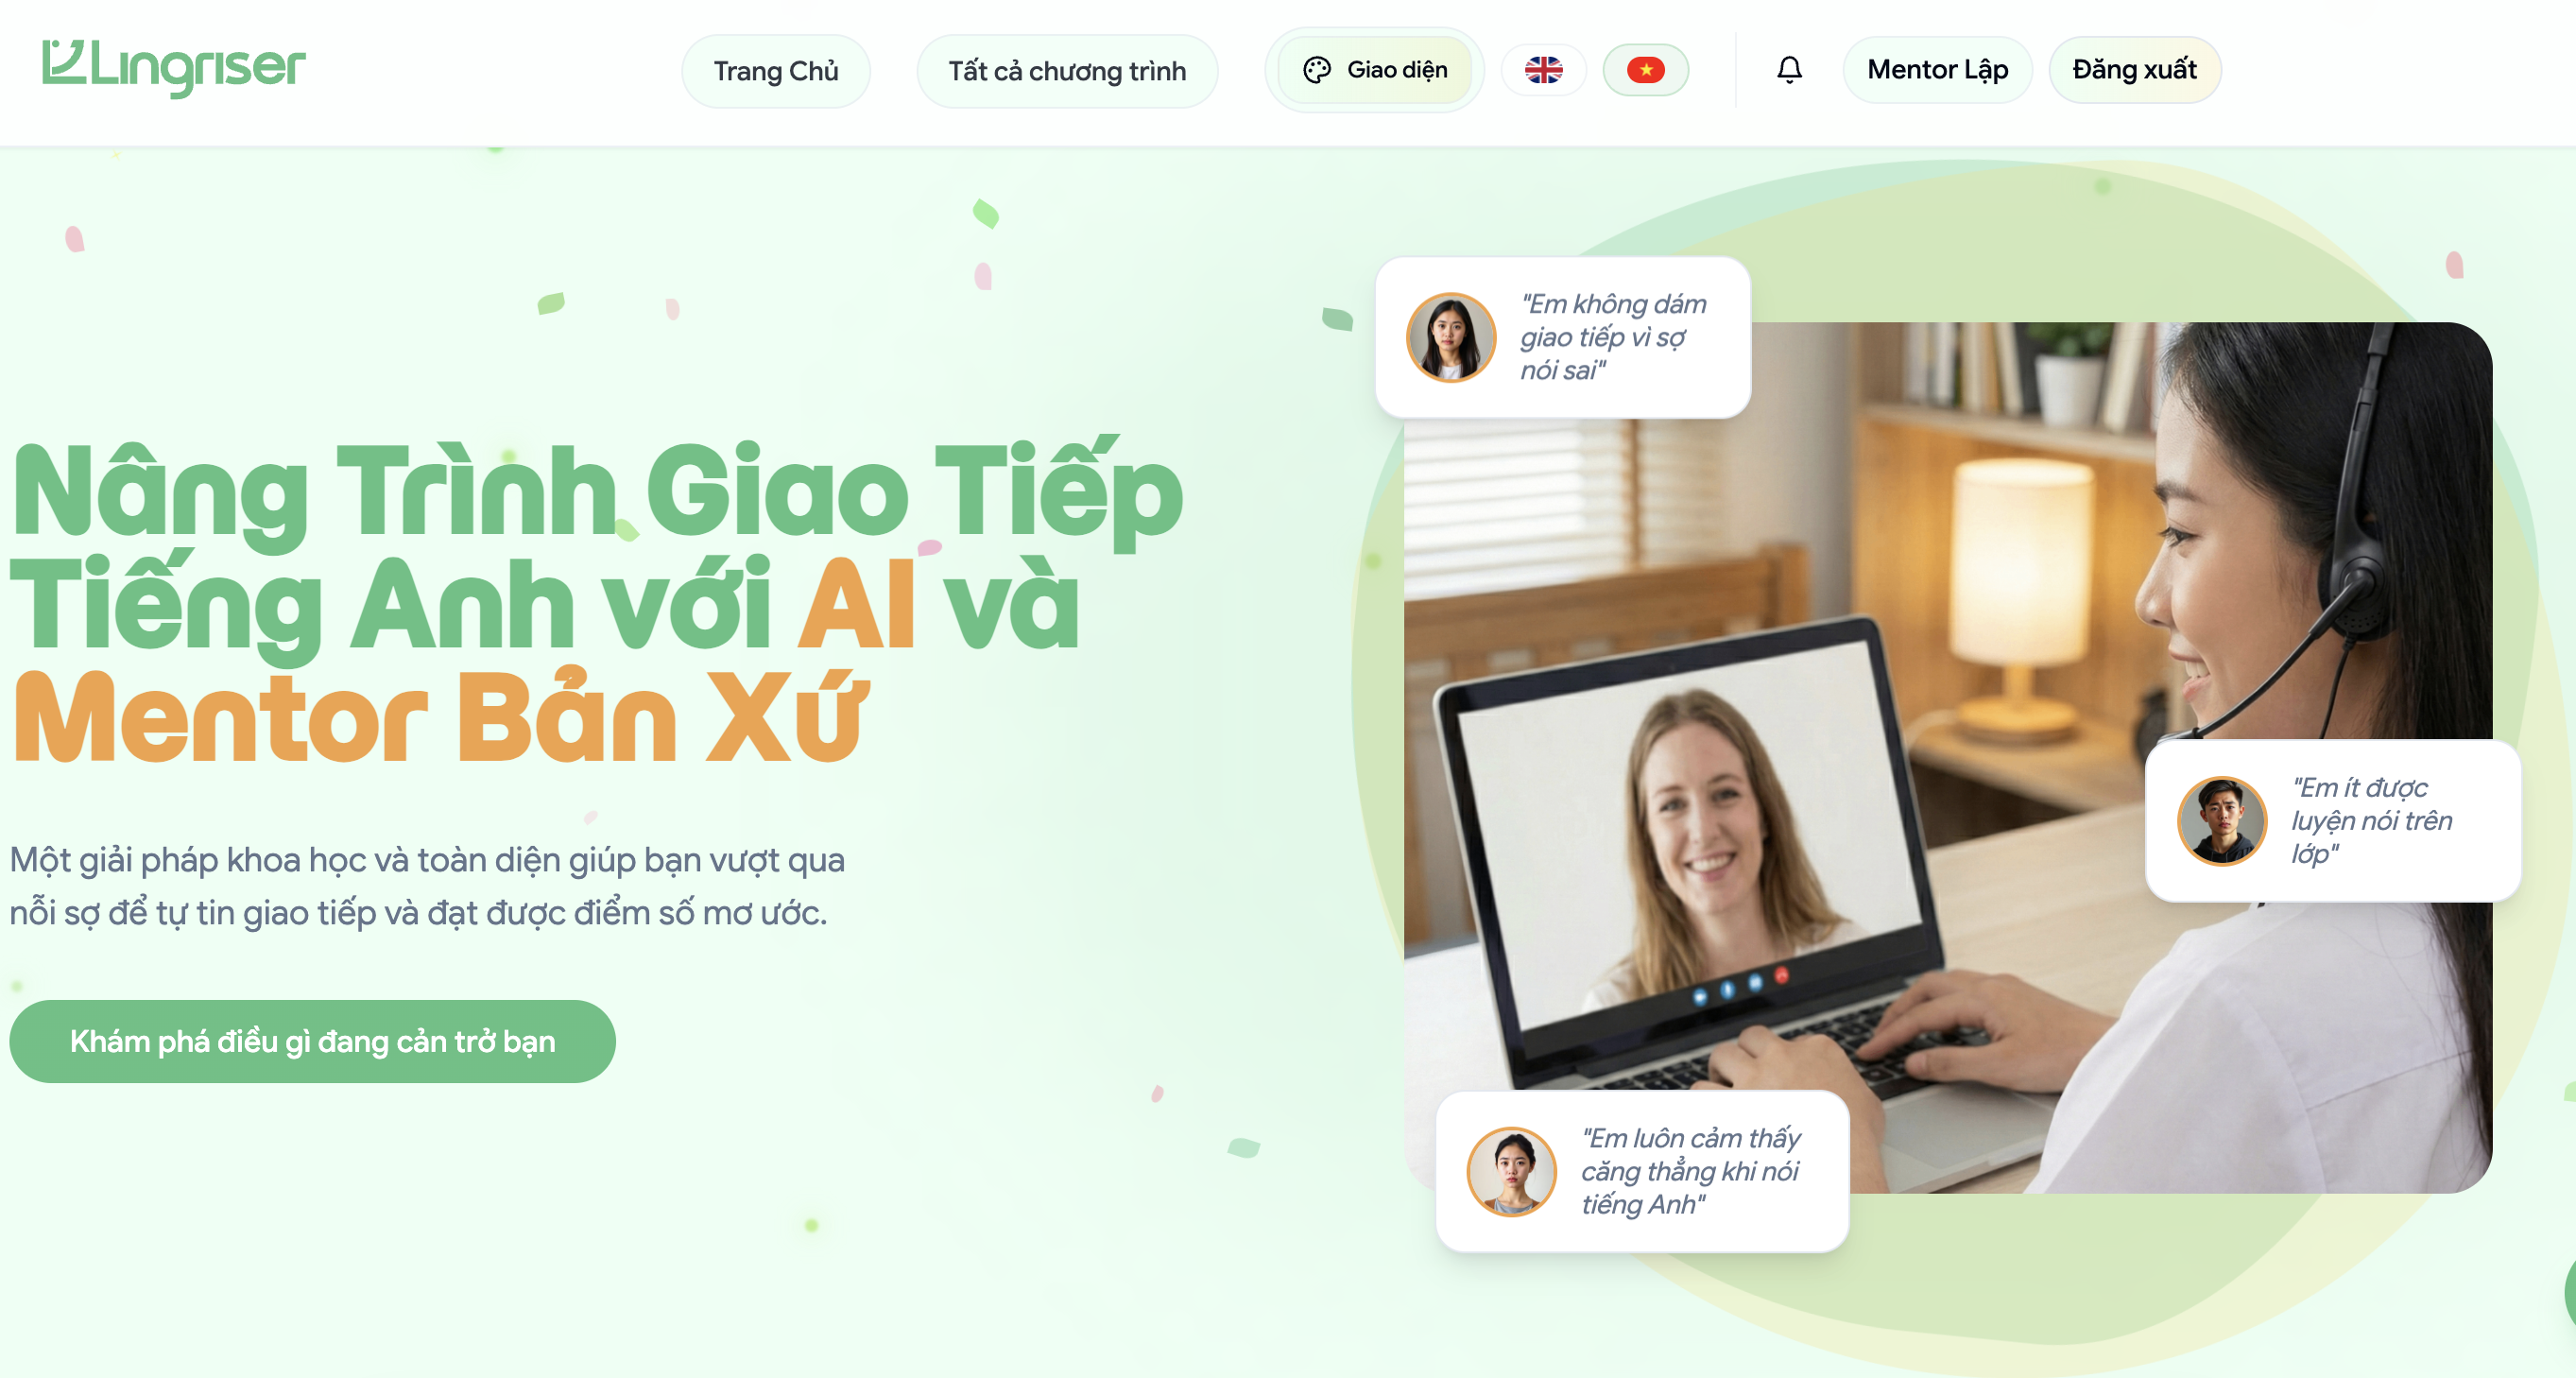
\includegraphics[width=\linewidth]{graphics/lingriser/dashboard}
    \captionsetup{skip=5pt}
    \caption{Giao diện luyện nói với AI của học sinh trên Lingriser}
\end{figure}

\textbf{Giao diện giáo viên} tập trung vào quản lý lịch buổi học và công cụ \textit{WeeklyFocus}. Sau buổi học thứ Hai, giáo viên nhập mục tiêu luyện nói cho từng module thông qua form này. Dữ liệu được lưu xuống backend và sau đó được mô-đun AI practice đọc lên để cá nhân hóa nội dung hội thoại, đồng thời hiển thị trong \textit{mentor brief} trước buổi video call cuối tuần.

\begin{figure}[H]
    \centering
    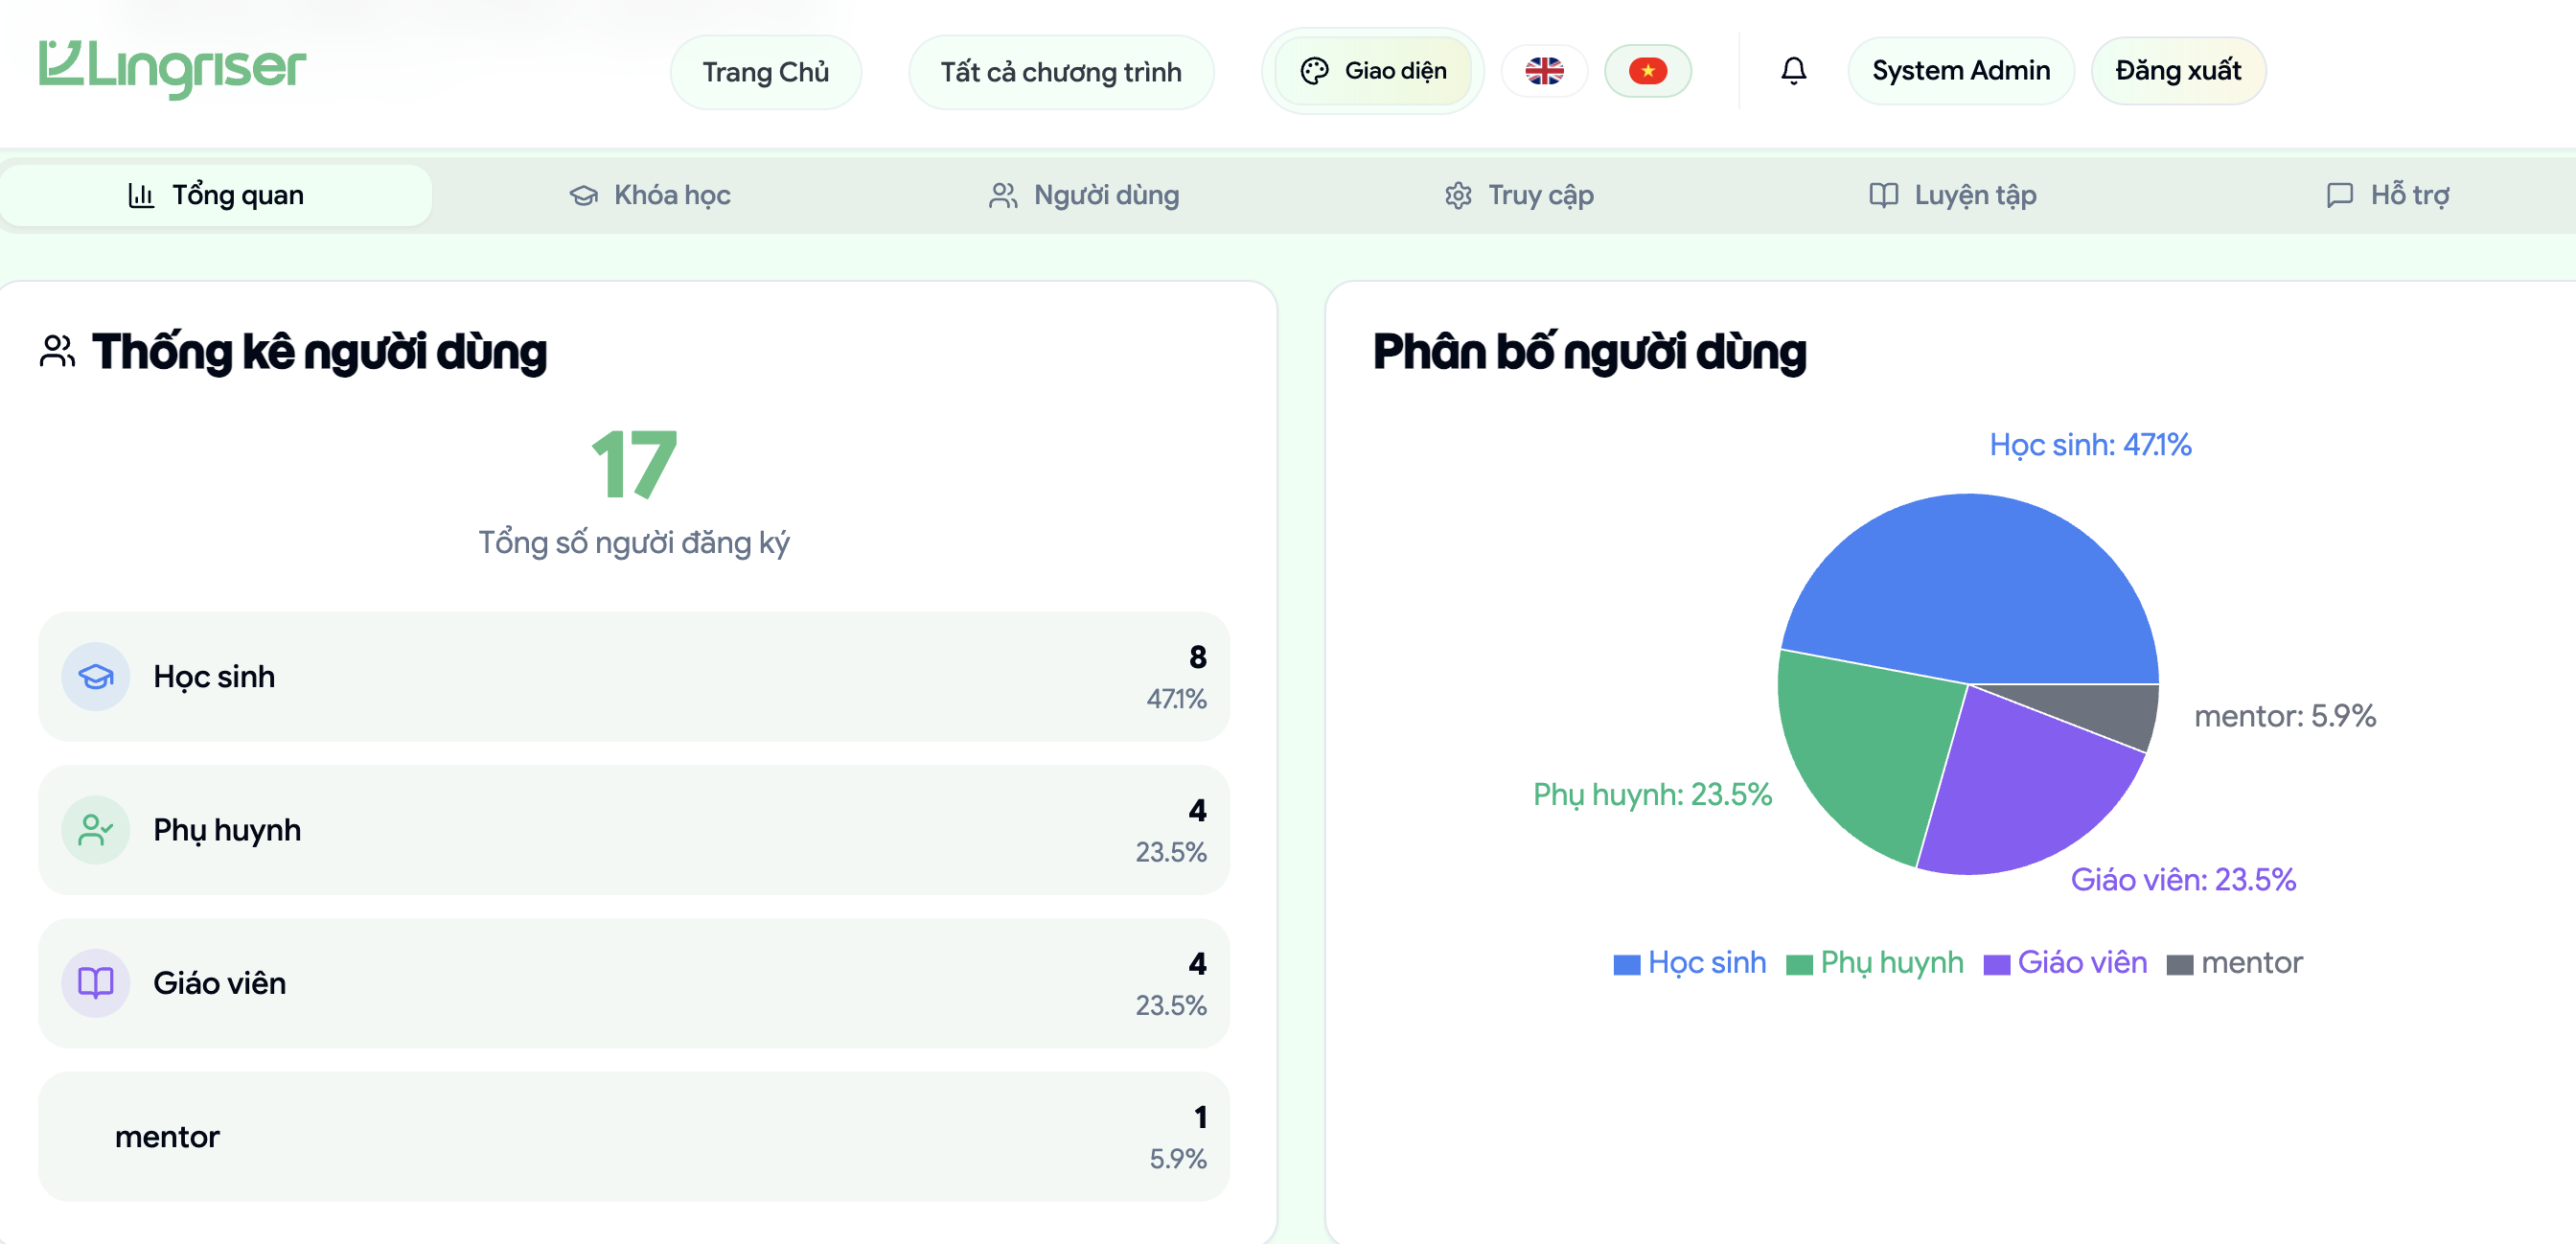
\includegraphics[width=0.9\linewidth]{graphics/lingriser/admin}
    \captionsetup{skip=5pt}
    \caption{Giao diện dashboard giáo viên với danh sách buổi học và công cụ đặt mục tiêu hằng tuần}
\end{figure}

\textbf{Giao diện đặt lịch và video call} cho phép học sinh chọn mentor, chọn khung giờ rảnh và xác nhận booking. Khi buổi học bắt đầu, hệ thống tạo link Google Meet tự động. Giáo viên/mentor có thể bắt đầu, kết thúc buổi học và gửi phản hồi ngay trên nền tảng; học sinh đánh giá buổi học sau khi kết thúc.

\begin{figure}[H]
    \centering
    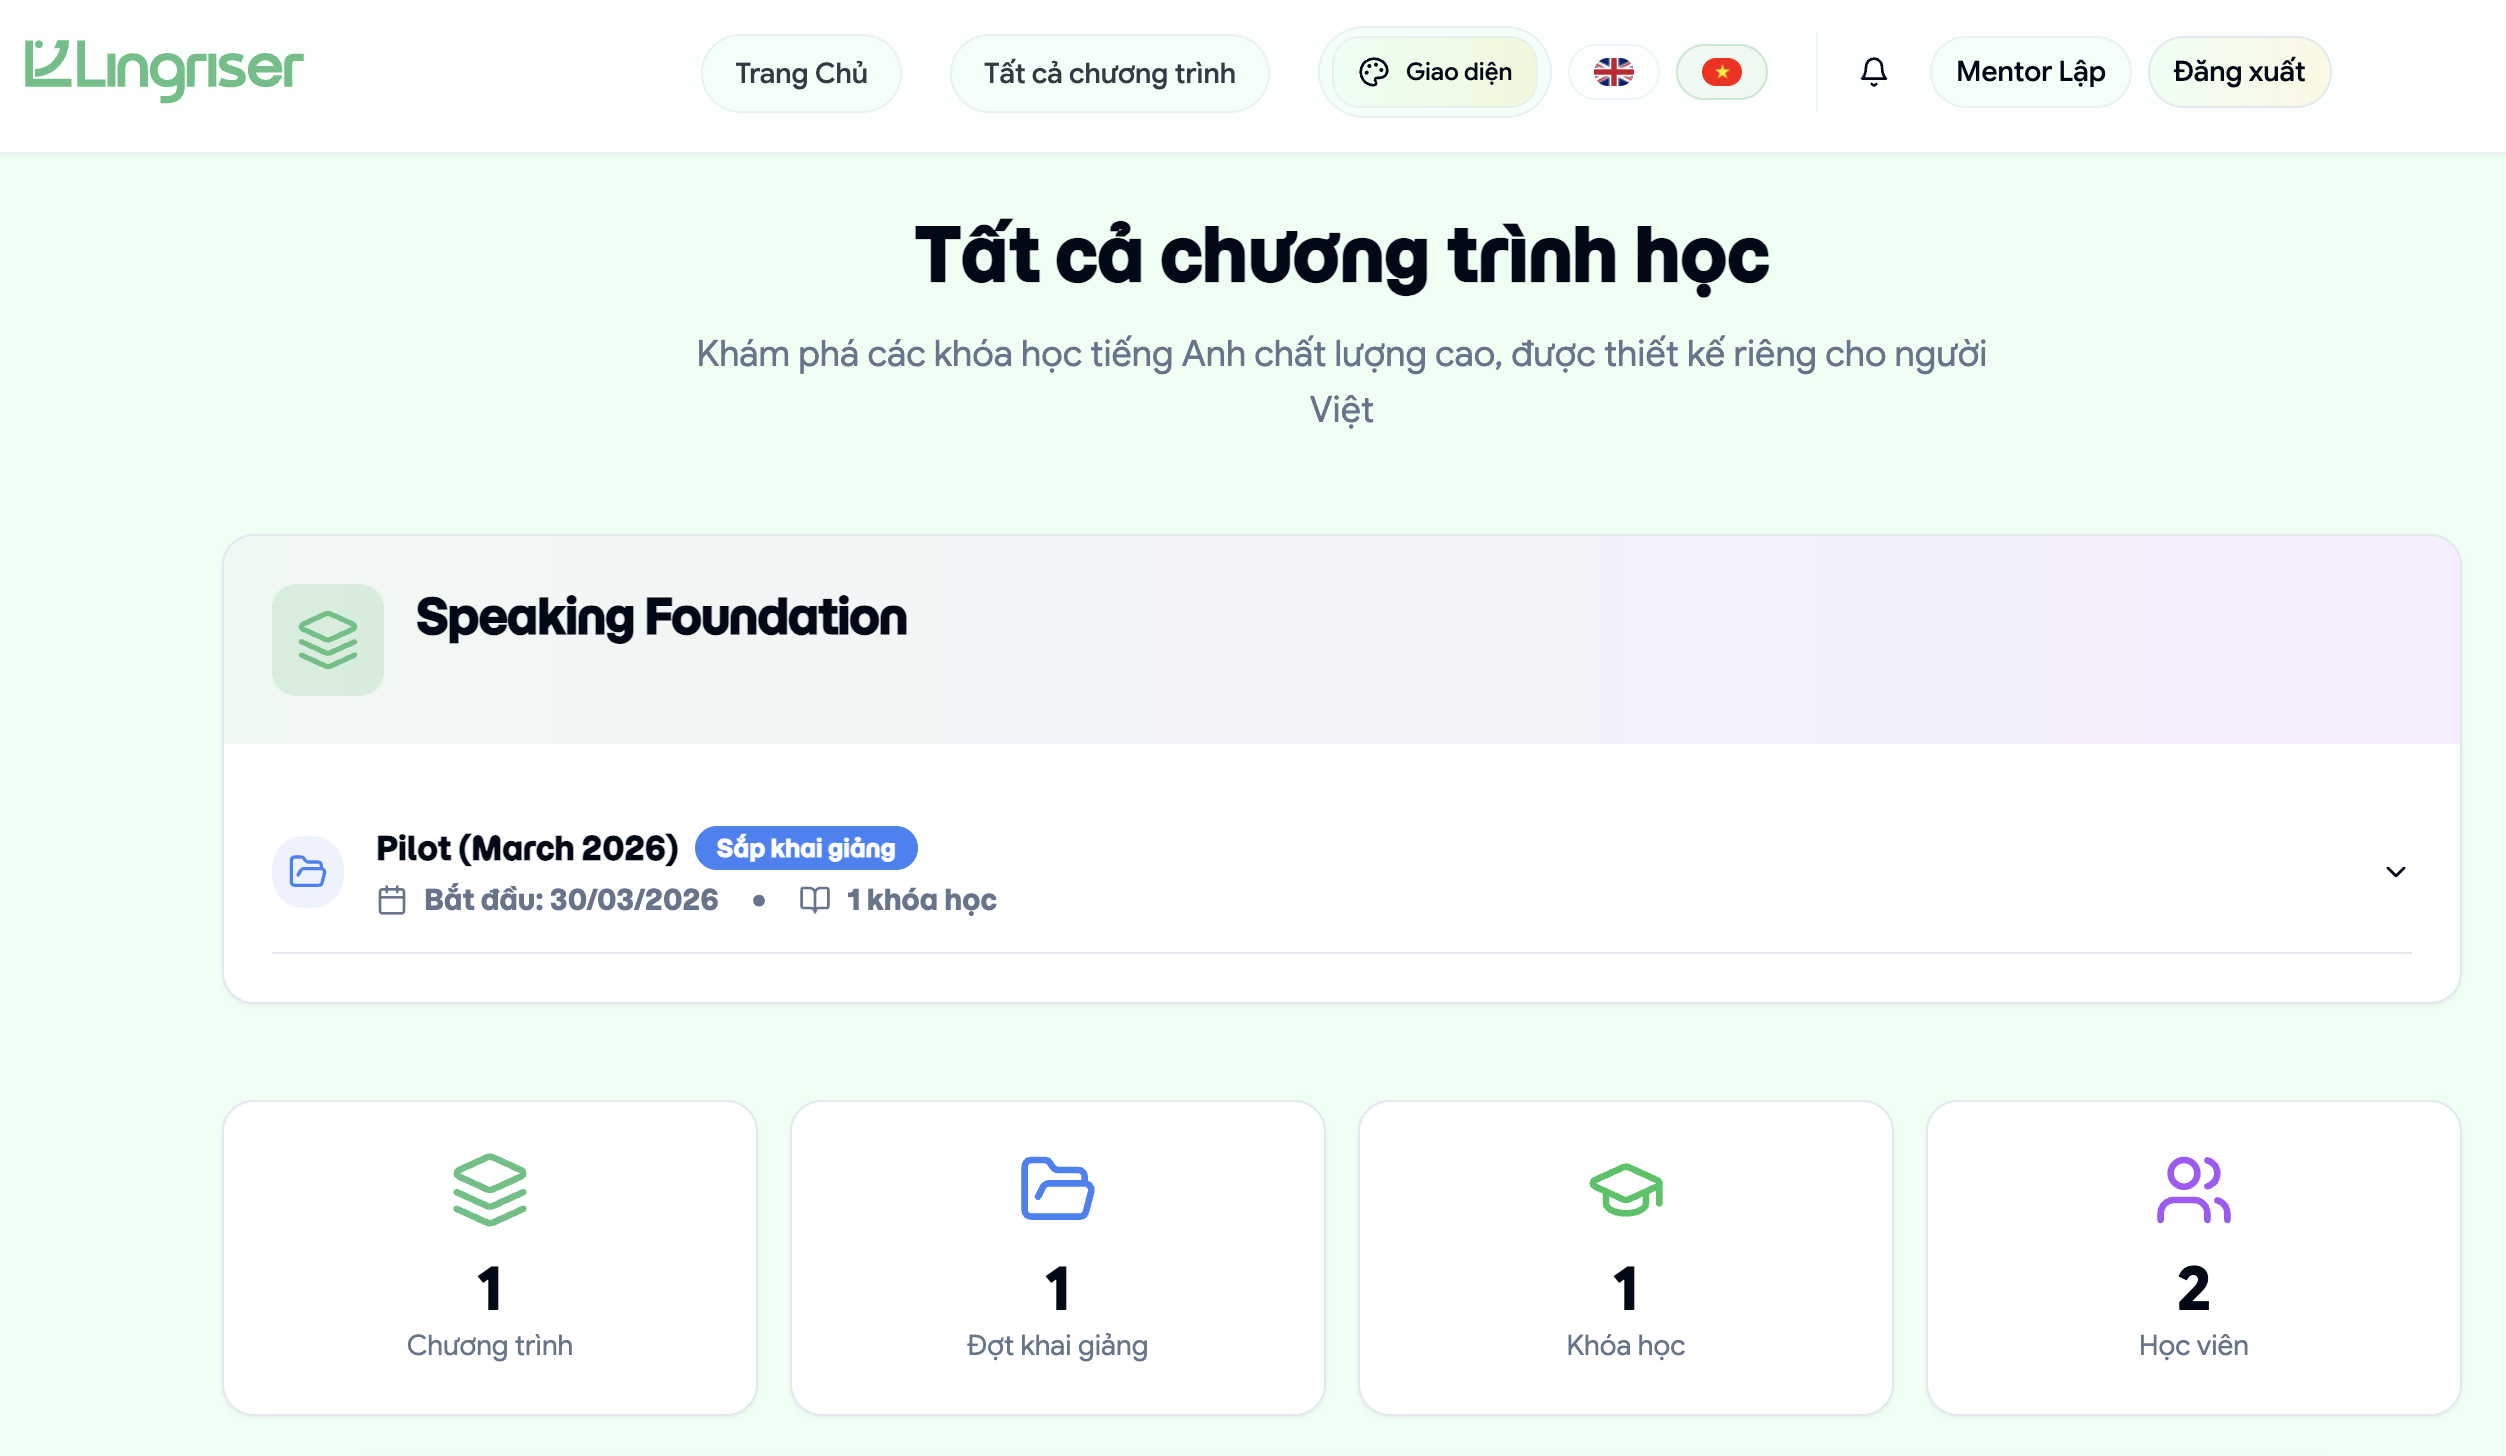
\includegraphics[width=0.9\linewidth]{graphics/lingriser/programs}
    \captionsetup{skip=5pt}
    \caption{Giao diện đặt lịch video call với mentor trên Lingriser}
\end{figure}

\subsection{Thiết kế cơ sở dữ liệu}

Lingriser sử dụng PostgreSQL (Neon Serverless) với schema được quản lý hoàn toàn bằng file SQL thuần — TypeORM được cấu hình \texttt{synchronize: false} để tránh auto-migration không kiểm soát.

\subsubsection{Nhóm bảng xác thực và hồ sơ người dùng}

Thiết kế sử dụng pattern \textbf{single-table base + profile extension}: bảng \texttt{users} lưu thông tin xác thực chung cho mọi vai trò gồm \texttt{email}, \texttt{password\_hash}, \texttt{phone}, \texttt{role} và \texttt{is\_locked}; còn mỗi vai trò có bảng profile riêng quan hệ 1:1 qua khóa ngoại \texttt{user\_id ON DELETE CASCADE}. Bảng \texttt{students} mở rộng với \texttt{grade}, \texttt{cefr\_level} và \texttt{assigned\_inperson\_teacher\_id}; bảng \texttt{teachers} thêm \texttt{teacher\_type} (\texttt{in\_person} / \texttt{video\_call} / \texttt{both}), \texttt{bio} và \texttt{specialties}.

Quan hệ phụ huynh--học sinh không lưu bằng FK trực tiếp mà qua bảng trung gian \texttt{account\_links(student\_id, linked\_user\_id, link\_type)}, cho phép một phụ huynh theo dõi nhiều học sinh và một học sinh có nhiều phụ huynh; đồng thời tái sử dụng cho quan hệ giáo viên--học sinh với \texttt{link\_type = 'teacher'}.

\subsubsection{Nhóm bảng chương trình học}

Bảng \texttt{courses} lưu thông tin khóa học gồm thời gian đăng ký, học phí (VND), trạng thái vòng đời (\texttt{upcoming → registration\_open → in\_progress → completed}) và lịch học thứ Hai. Mỗi course có đúng 8 bản ghi \texttt{modules}, ràng buộc bởi \texttt{UNIQUE(course\_id, module\_number)} và \texttt{CHECK(module\_number BETWEEN 1 AND 8)}. Mỗi module lưu \texttt{week\_start\_date}/\texttt{week\_end\_date} và ba cột JSONB chứa nội dung tương ứng ba tầng học tập: \texttt{monday\_content}, \texttt{ai\_practice\_content} và \texttt{teacher\_session\_content}. Bảng \texttt{enrollments} ghi nhận đăng ký của học sinh, theo dõi \texttt{current\_module\_number} và trạng thái thanh toán.

\subsubsection{Nhóm bảng theo dõi hoạt động học tập}

Bảng \texttt{learning\_history} là trung tâm ghi nhận mọi hoạt động của học sinh, phân biệt qua cột \texttt{activity\_type} với ba giá trị: \texttt{in\_person\_class}, \texttt{ai\_practice} và \texttt{video\_call}. Mỗi bản ghi gắn với \texttt{student\_id}, \texttt{module\_id}, khoảng thời gian thực tế và FK tùy chọn \texttt{booking\_id} (chỉ dành cho \texttt{video\_call}).

Bảng \texttt{ai\_feedback} có quan hệ 1:1 với \texttt{learning\_history} dành riêng cho buổi AI practice. Ngoài \texttt{feedback\_text}, Migration 009 bổ sung bốn trường analytics: \texttt{speech\_to\_text} (bản phiên âm đầy đủ), \texttt{response\_duration} (giây trung bình mỗi lượt), \texttt{pause\_detection JSONB} (kết quả phân tích khoảng ngừng gồm \texttt{has\_pause}, \texttt{pause\_count}, \texttt{pause\_turns[]}) và \texttt{session\_length} (số lượt hội thoại).

\subsubsection{Bảng booking và tích hợp Google Meet}

Bảng \texttt{bookings} quản lý toàn bộ vòng đời buổi video call qua hai enum độc lập: \texttt{status} (\texttt{confirmed / completed / cancelled / no\_show}) theo dõi kết quả cuối cùng, còn \texttt{meeting\_status} (\texttt{pending / in\_progress / ended}) theo dõi trạng thái thời gian thực trong buổi học. \texttt{meeting\_link} và \texttt{google\_event\_id} được thêm qua Migration 004 khi tích hợp Google Calendar. Migration 007 đưa \texttt{teacher\_feedback}, \texttt{student\_rating} (1--5) và \texttt{student\_comment} vào thẳng bảng \texttt{bookings} thay vì tạo bảng phụ. OAuth tokens của giáo viên lưu riêng trong \texttt{teacher\_google\_tokens} với \texttt{access\_token}, \texttt{refresh\_token} và \texttt{expires\_at}.

\subsubsection{Bảng \texttt{weekly\_focus}}

Đây là bảng then chốt liên kết ba tầng học tập. Ràng buộc \texttt{UNIQUE(module\_id, teacher\_id)} đảm bảo mỗi giáo viên chỉ có một bản mục tiêu cho mỗi module, và \texttt{WeeklyFocusService.createOrUpdate()} tận dụng constraint này để upsert thay vì insert/update riêng. Trường đặc biệt là \texttt{speaking\_goals TEXT[]} — kiểu mảng native PostgreSQL lưu trực tiếp danh sách mục tiêu dạng chuỗi. TypeORM ánh xạ cột này thành \texttt{string[]} trong TypeScript và truyền thẳng vào \texttt{buildSystemPrompt()} mỗi khi học sinh bắt đầu phiên luyện AI.

\subsubsection{Chỉ mục hiệu năng}

Schema định nghĩa 15 index phủ các truy vấn thường xuyên nhất. Nhóm index quan trọng nhất thuộc về bảng \texttt{bookings} với ba index riêng biệt trên \texttt{student\_id}, \texttt{booking\_date} và \texttt{status} — vì trang lịch của mentor và học sinh phải lọc đồng thời theo cả ba chiều. Bảng \texttt{learning\_history} có index trên \texttt{student\_id} và \texttt{activity\_type} để phục vụ truy vấn thống kê tuần của phụ huynh mà không cần full table scan. Bảng \texttt{users} được index trên \texttt{email}, \texttt{phone} và \texttt{role} để tăng tốc đăng nhập và lọc người dùng theo vai trò trong admin dashboard.

\subsection{Pipeline dữ liệu WeeklyFocus → AI Practice → Mentor Brief}

Đây là luồng dữ liệu kỹ thuật quan trọng nhất của Lingriser, kết nối ba tầng hoạt động học tập thành một chu trình có trạng thái:

\begin{enumerate}
    \item \textbf{Giáo viên thiết lập mục tiêu:} Giao diện quản lý gửi một payload chứa định danh học phần, giáo viên, chủ đề và danh sách mục tiêu luyện nói. Ở lớp backend, hệ thống thực hiện cơ chế \textit{upsert} dựa trên ràng buộc duy nhất (unique constraint) của học phần và giáo viên để cập nhật hoặc tạo mới bản ghi. Danh sách mục tiêu được định dạng và lưu trữ dưới dạng cấu trúc mảng trong cơ sở dữ liệu.

    \item \textbf{Tích hợp mục tiêu vào phiên AI:} Khi người dùng bắt đầu phiên luyện tập, client truyền danh sách mục tiêu này trong payload yêu cầu khởi tạo hội thoại. Lớp dịch vụ chịu trách nhiệm xây dựng \textit{system prompt} bằng cách nhúng (embed) mảng mục tiêu vào một khối định hướng cục bộ. Mô hình ngôn ngữ lớn sau đó sử dụng khối ngữ cảnh này như một tập luật ràng buộc để điều hướng nội dung giao tiếp bám sát thiết kế sư phạm.

    \item \textbf{Xử lý và lưu trữ kết quả luyện tập:} Kết thúc buổi thực hành, hệ thống khởi tạo một bản ghi lịch sử học tập định danh cho hoạt động luyện AI. Kế tiếp, một luồng phân tích tiến hành xử lý bản phiên âm (transcript) để trích xuất các tham số kỹ thuật như điểm ngắt nghỉ (pause detection) và thời lượng phản hồi (response duration). Các chỉ số đánh giá này được lưu trữ vào một thực thể dữ liệu độc lập, liên kết với bản ghi lịch sử gốc thông qua khóa ngoại (foreign key).

    \item \textbf{Tổng hợp tóm tắt (Mentor Brief):} Để hỗ trợ mentor trước buổi học đồng bộ, hệ thống cung cấp một API truy xuất dữ liệu tóm tắt. Backend thực thi các truy vấn song song nhằm thu thập thông tin từ ba cấu trúc thực thể: (a) truy xuất mục tiêu tuần hiện tại, (b) thực hiện phép tính gộp (aggregation) trên bảng lịch sử để xác định tần suất luyện tập, và (c) thực hiện phép kết nối (JOIN) để lấy dữ liệu đánh giá của phiên gần nhất. Toàn bộ thông tin được đóng gói thành một response duy nhất, giúp tái tạo toàn diện bối cảnh học tập của học viên.
\end{enumerate}

\begin{figure}[H]
    \centering
    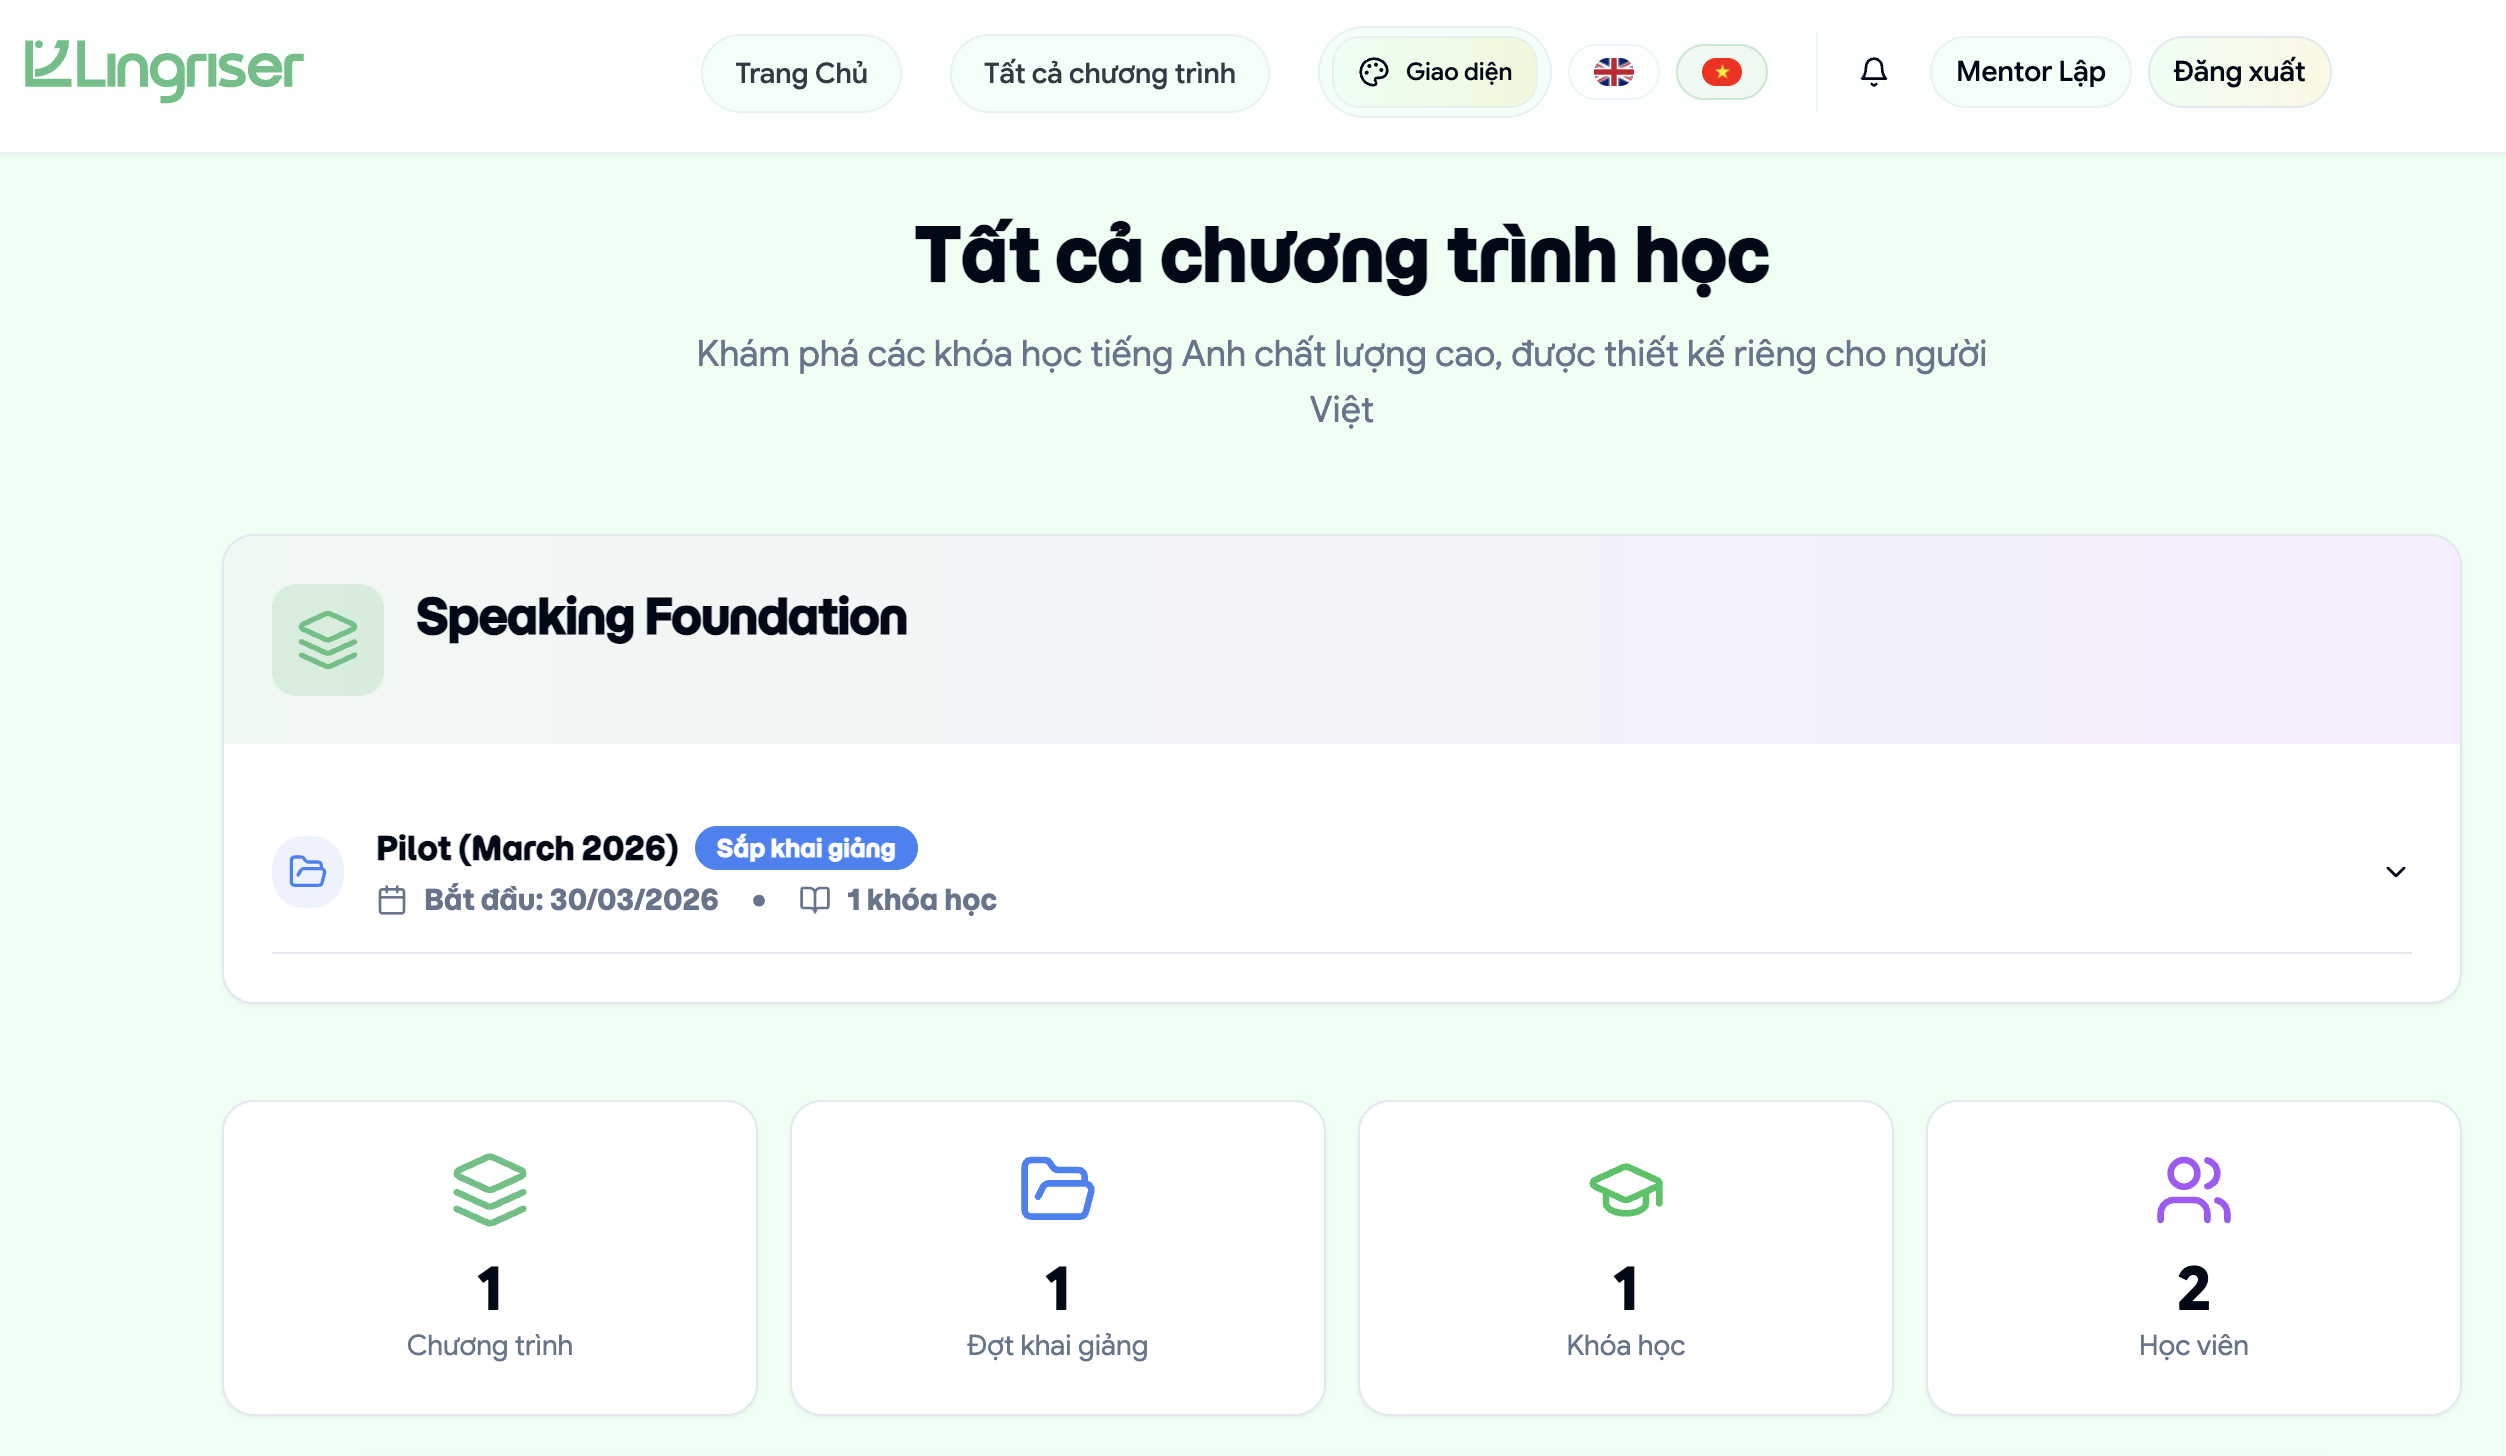
\includegraphics[width=0.95\linewidth]{graphics/lingriser/programs}
    \captionsetup{skip=5pt}
    \caption{Quản lý chương trình học và tiến trình theo module trong Lingriser}
\end{figure}

Toàn bộ pipeline này không có bước thủ công nào giữa các tầng — dữ liệu từ giáo viên tự động xuất hiện trong AI practice, và kết quả AI practice tự động tổng hợp thành mentor brief, nhờ các foreign key và truy vấn có cấu trúc trên cùng một PostgreSQL database.

\subsection{Cơ chế theo dõi tiến độ học tập dành cho phụ huynh}

Phụ huynh là vai trò đặc biệt trong Lingriser: họ không trực tiếp tham gia học tập nhưng được cấp quyền đọc toàn bộ dữ liệu của con thông qua một lớp truy cập riêng. Cơ chế này được thiết kế có chủ đích — không để phụ huynh can thiệp vào luồng AI, mà để dữ liệu do AI tạo ra trở nên có giá trị hơn bằng cách đưa gia đình vào vòng quan sát.

\subsubsection{Cơ chế liên kết tài khoản}

Quan hệ phụ huynh--học sinh không lưu bằng foreign key trực tiếp mà qua bảng trung gian \texttt{account\_links} với ba cột chính: \texttt{student\_id}, \texttt{linked\_user\_id} và \texttt{link\_type} (nhận giá trị \texttt{'parent'} hoặc \texttt{'teacher'}). Ràng buộc \texttt{UNIQUE(student\_id, linked\_user\_id)} ngăn trùng liên kết. Thiết kế này cho phép một phụ huynh theo dõi nhiều học sinh (nhiều bản ghi cùng \texttt{linked\_user\_id}), đồng thời một học sinh có thể được liên kết với nhiều phụ huynh. Khi truy vấn danh sách con của phụ huynh, \texttt{ParentsService} JOIN qua bảng này lọc theo \texttt{link\_type = 'parent'} và \texttt{is\_locked = FALSE} để loại bỏ tài khoản bị khóa.

\subsubsection{Kiểm soát truy cập theo phụ huynh}

Toàn bộ các phương thức trong \texttt{ParentsService} đều thực hiện bước xác minh quyền sở hữu trước khi trả dữ liệu: gọi \texttt{getChildren(parentId)} để lấy danh sách học sinh được liên kết, sau đó kiểm tra \texttt{children.some(c => c.id === studentId)}. Nếu học sinh không thuộc phụ huynh đó, hệ thống ném \texttt{NotFoundException} ngay tại service layer, không để lọt xuống database. Đây là lớp bảo vệ bổ sung sau JWT auth guard, đảm bảo phụ huynh không thể truy cập dữ liệu học sinh của gia đình khác dù biết \texttt{studentId}.

\subsubsection{Thống kê AI practice theo tuần}

Đây là dữ liệu trực quan nhất mà phụ huynh có thể theo dõi — số buổi luyện AI và tổng phút luyện tập mỗi tuần. \texttt{getAIPracticeWeeklyStats()} thực hiện truy vấn tổng hợp trên PostgreSQL với \texttt{DATE\_TRUNC('week', start\_time)} để nhóm theo tuần, \texttt{COUNT(*)} đếm số buổi và \texttt{EXTRACT(EPOCH FROM (end\_time - start\_time)) / 60} tính tổng phút; lọc theo \texttt{student\_id}, \texttt{activity\_type = 'ai\_practice'} và khoảng \texttt{N} tuần gần nhất.

Kết quả thô chỉ chứa các tuần có dữ liệu. Backend thực hiện bước \textbf{fill missing weeks}: duyệt vòng lặp từ tuần cũ nhất đến hiện tại (mặc định 8 tuần), căn chỉnh về thứ Hai của từng tuần, ghép với kết quả truy vấn nếu khớp, ngược lại điền \texttt{sessions = 0} và \texttt{minutes = 0}. Kết quả cuối cùng là mảng đủ 8 phần tử sẵn sàng render trực tiếp thành biểu đồ cột trên frontend (sử dụng Recharts).

\subsubsection{Xác định module hiện tại theo ngày thực tế}

Khi phụ huynh xem thông tin đăng ký của con, hàm \texttt{computeCurrentModuleNumber()} tự động tính module đang được học bằng cách duyệt qua danh sách module và so sánh ngày hiện tại với \texttt{week\_start\_date} và \texttt{week\_end\_date} của từng module. Nếu không thuộc khoảng nào (trước khi khóa học bắt đầu hoặc sau khi kết thúc), hàm trả về module đầu tiên hoặc module cuối. Trường \texttt{current\_module\_number} được tính động tại mỗi request thay vì lưu cứng trong database, đảm bảo thông tin luôn chính xác mà không cần scheduled job cập nhật.

\subsubsection{Video tiến trình trước và sau khoá học}

Ngoài dữ liệu số, Lingriser còn cho phép học sinh upload video tự quay trước khi bắt đầu (\texttt{video\_type = 'before'}) và sau khi kết thúc (\texttt{video\_type = 'after'}) khoá học. Video được lưu trên AWS S3 với tiền tố \texttt{lingriser/student-videos/}; bảng \texttt{student\_videos} chỉ lưu URL và metadata. Phụ huynh có thể xem cả hai video qua endpoint \texttt{/progress-videos}, tạo bằng chứng hữu hình về sự tiến bộ của con trong suốt 8 tuần học.

\begin{figure}[H]
    \centering
    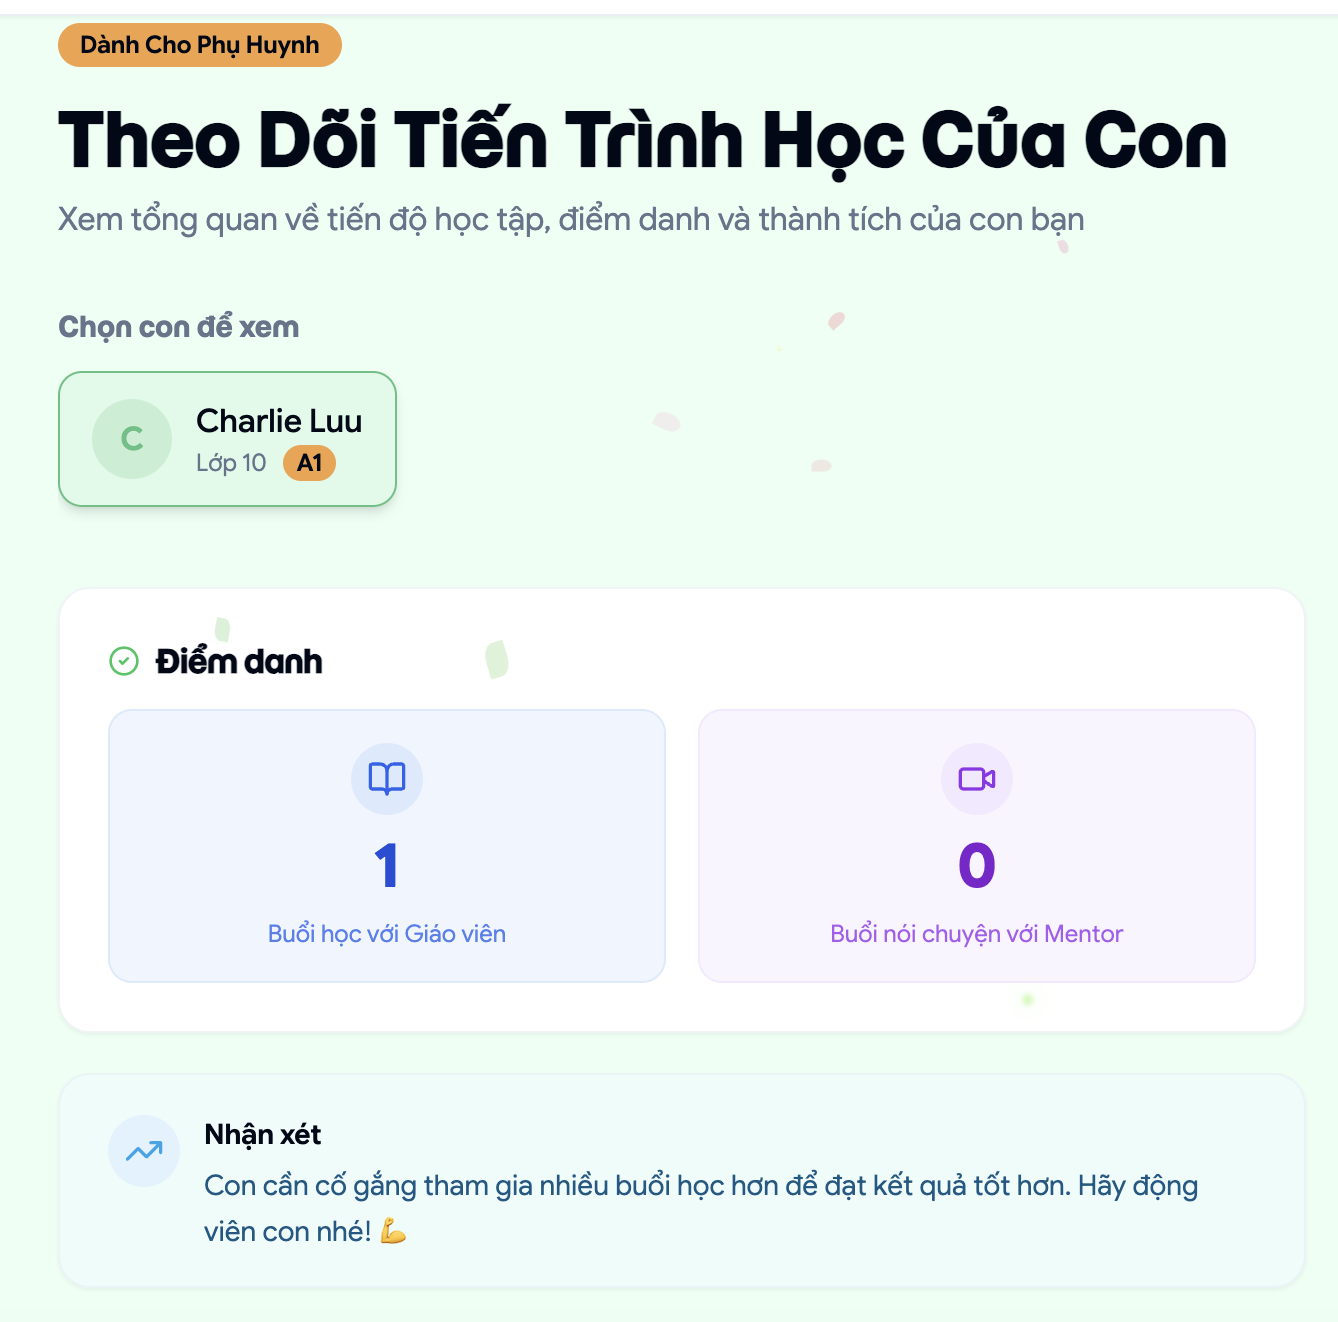
\includegraphics[width=0.88\linewidth]{graphics/lingriser/parents}
    \captionsetup{skip=5pt}
    \caption{Giao diện dashboard phụ huynh — theo dõi tiến trình AI practice và lịch học của con}
\end{figure}


\subsection{Giá trị của Lingriser đối với bài toán Speaking}
So với một hệ thống chấm điểm Speaking thuần túy, Lingriser giải quyết bài toán rộng hơn: duy trì thói quen luyện nói liên tục trong bối cảnh học sinh Việt Nam thường thiếu môi trường sử dụng tiếng Anh. Giá trị lớn nhất của nền tảng không nằm ở một mô hình đơn lẻ, mà ở cách kết hợp AI hội thoại, phiên âm, TTS, quản lý tiến trình và định hướng sư phạm thành một trải nghiệm thống nhất. Điều này giúp người học nhận được phản hồi thường xuyên, có động lực quay lại luyện tập và có sự kết nối giữa tự học với hoạt động dạy học có người hướng dẫn.

Từ góc độ kiến trúc hệ thống, Lingriser cũng cho thấy hướng triển khai thực tế của các tính năng AI cho Speaking trên nền web: frontend cung cấp giao diện luyện tập trực quan, backend điều phối logic nghiệp vụ và xác thực, còn lớp AI đảm nhiệm các tác vụ ngôn ngữ và giọng nói. Đây là một minh chứng cụ thể cho khả năng tích hợp AI vào sản phẩm giáo dục theo hướng vừa khả thi về kỹ thuật, vừa hợp lý về trải nghiệm người dùng.

\section{Tính năng AI cho Writing}
Bên cạnh mô-đun Speaking, hệ thống được mở rộng thêm mô-đun AI cho Writing nhằm hỗ trợ người học trong bài toán luyện viết học thuật theo định dạng IELTS. Khác với Speaking, nơi trọng tâm là xử lý hội thoại và tín hiệu âm thanh theo thời gian gần thực, mô-đun Writing tập trung vào phân tích văn bản đầu vào, ước lượng chất lượng bài viết và sinh phản hồi cải thiện theo từng tiêu chí chấm điểm. Trong đồ án này, nhóm lựa chọn hướng xây dựng một mô hình Writing chuyên biệt dựa trên \textbf{Phi-3-mini-4k-instruct}, sau đó fine-tune trên tập dữ liệu IELTS Writing đã được chuẩn hóa và triển khai như một service độc lập để tích hợp vào hệ thống luyện thi tiếng Anh.

\subsection{Mục tiêu của mô-đun Writing}
Mục tiêu chính của mô-đun là tự động hóa một phần quá trình đánh giá bài viết và cung cấp phản hồi học tập hữu ích cho người dùng. Cụ thể, hệ thống được thiết kế để:
\begin{itemize}
    \item Dự đoán \textbf{Overall Band Score} cho bài viết IELTS Writing.
    \item Chấm đồng thời \textbf{4 tiêu chí thành phần} gồm Task Achievement/Response, Coherence \& Cohesion, Lexical Resource và Grammatical Range \& Accuracy.
    \item Sinh \textbf{nhận xét chi tiết} dưới dạng đoạn văn, chỉ ra điểm mạnh, điểm yếu và hướng cải thiện.
    \item Tạo nền tảng để tích hợp AI chấm bài Writing trực tiếp vào hệ thống web luyện thi của nhóm.
\end{itemize}

\subsection{Bài toán và định hướng mô hình}
Ở góc độ kỹ thuật, đây là bài toán \textit{instruction tuning} cho mô hình ngôn ngữ lớn với đầu vào là \textbf{đề bài IELTS Writing} và \textbf{bài viết của người học}, còn đầu ra là một phản hồi có cấu trúc gồm điểm số và nhận xét. Mô hình không chỉ thực hiện một tác vụ đơn lẻ mà kết hợp đồng thời ba lớp nhiệm vụ: \textit{scoring}, \textit{feedback generation} và \textit{error explanation}. 

Nhóm lựa chọn \textbf{Phi-3-mini-4k-instruct} làm mô hình nền vì mô hình này có quy mô vừa phải, phù hợp với tài nguyên tính toán sẵn có trên Kaggle GPU, đồng thời vẫn giữ được khả năng sinh ngôn ngữ đủ tốt cho bài toán đánh giá viết. Ngoài ra, kiến trúc này tương thích tốt với các kỹ thuật fine-tune tiết kiệm tài nguyên như \textit{QLoRA}, cho phép nhóm huấn luyện mô hình trong điều kiện VRAM hạn chế nhưng vẫn đạt được chất lượng đầu ra chấp nhận được.

Trong hệ thống thực tế, mô hình đóng vai trò là thành phần suy luận cho chức năng Writing trên web: backend nhận bài viết từ người dùng, chuẩn hóa request, chuyển tới service chứa mô hình đã train, sau đó trả về điểm và phản hồi để hiển thị trên giao diện.

\subsection{Thu thập và xây dựng dữ liệu huấn luyện}

\subsubsection{Nguồn dữ liệu}
Dữ liệu huấn luyện được xây dựng từ các nguồn phục vụ ôn luyện IELTS Writing phổ biến, sau đó được chuẩn hóa và đưa về cùng một định dạng để sử dụng trong quá trình huấn luyện. Ba nguồn chính được sử dụng gồm:
\begin{itemize}
    \item \textbf{IELTS Writing Dataset trên Kaggle}: cung cấp tập dữ liệu có cấu trúc, thuận tiện cho việc xử lý tự động và huấn luyện mô hình.
    \item \textbf{chillies/IELTS-writing-task-2-evaluation trên Hugging Face}: cung cấp thêm một nguồn dữ liệu chuyên biệt cho bài toán IELTS Writing Task 2. Theo mô tả của tác giả: \textit{``The essays are written by real test takers, and the band scores are assigned by expert examiners. However, the evaluation/feedback is generated by Gemini Pro based on prompts that I created.''} Nguồn dữ liệu này đặc biệt hữu ích vì kết hợp giữa bài viết thực của thí sinh, band score do expert examiner gán và phần evaluation/feedback được tạo có cấu trúc để phục vụ các tác vụ huấn luyện mô hình.
    \item \textbf{IELTS Mentor}: cung cấp nhiều đề bài, bài mẫu và bài viết được chấm điểm, hữu ích cho việc bổ sung dữ liệu theo đúng ngữ cảnh luyện thi.
    \item \textbf{IELTS Blog}: bổ sung thêm các bài viết và nhận xét từ môi trường ôn luyện thực tế, giúp tăng tính đa dạng của tập dữ liệu.
\end{itemize}

Sau khi được tổng hợp và chuẩn hóa, bốn nguồn này tạo thành tập dữ liệu huấn luyện scored gồm \textbf{9872 bản ghi bài viết}. Việc kết hợp dữ liệu từ nhiều website ôn luyện khác nhau giúp tăng độ đa dạng về chủ đề, dạng bài, độ dài bài viết, band điểm và phong cách phản hồi.

\begin{figure}[H]
    \centering
    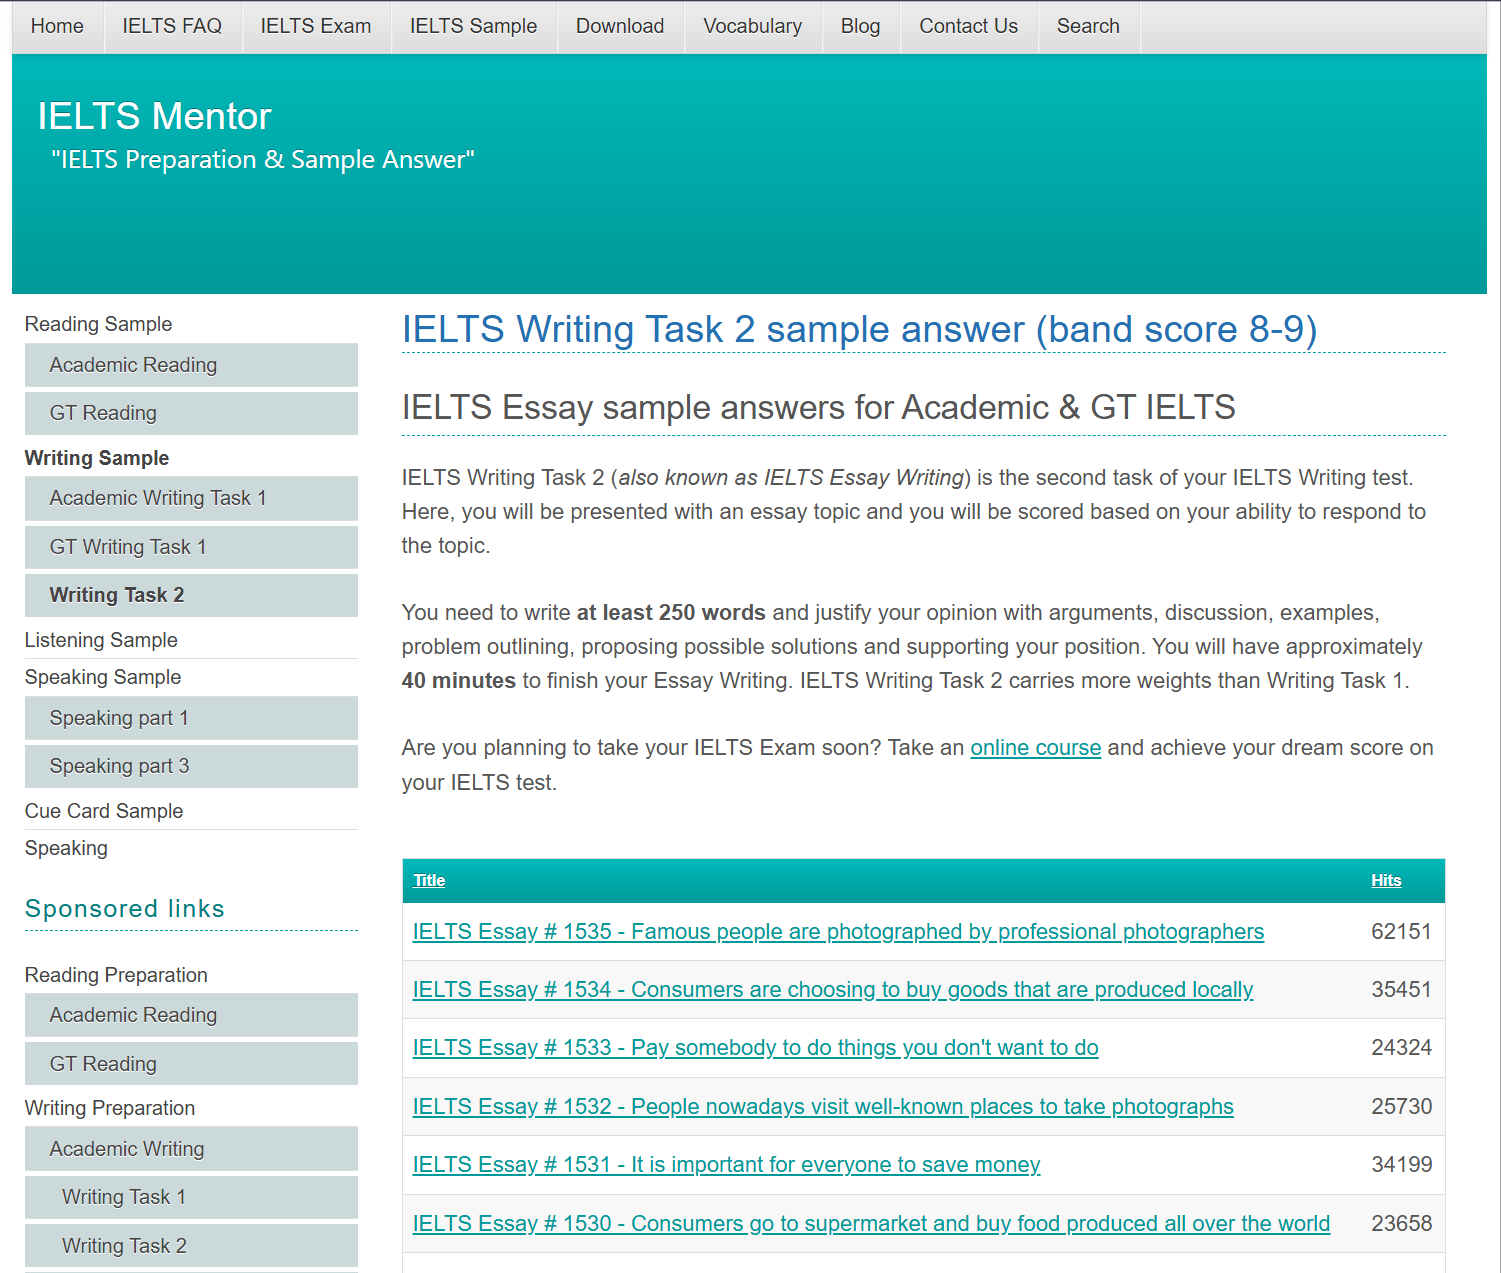
\includegraphics[width=0.92\linewidth]{graphics/writing/ielts_mentor}
    \captionsetup{skip=5pt}
    \caption{Trang web IELTS Mentor cung cấp nhiều đề bài, bài mẫu và bài viết được chấm điểm}
    \label{fig:data-source-kaggle}
\end{figure}

\begin{figure}[H]
    \centering
    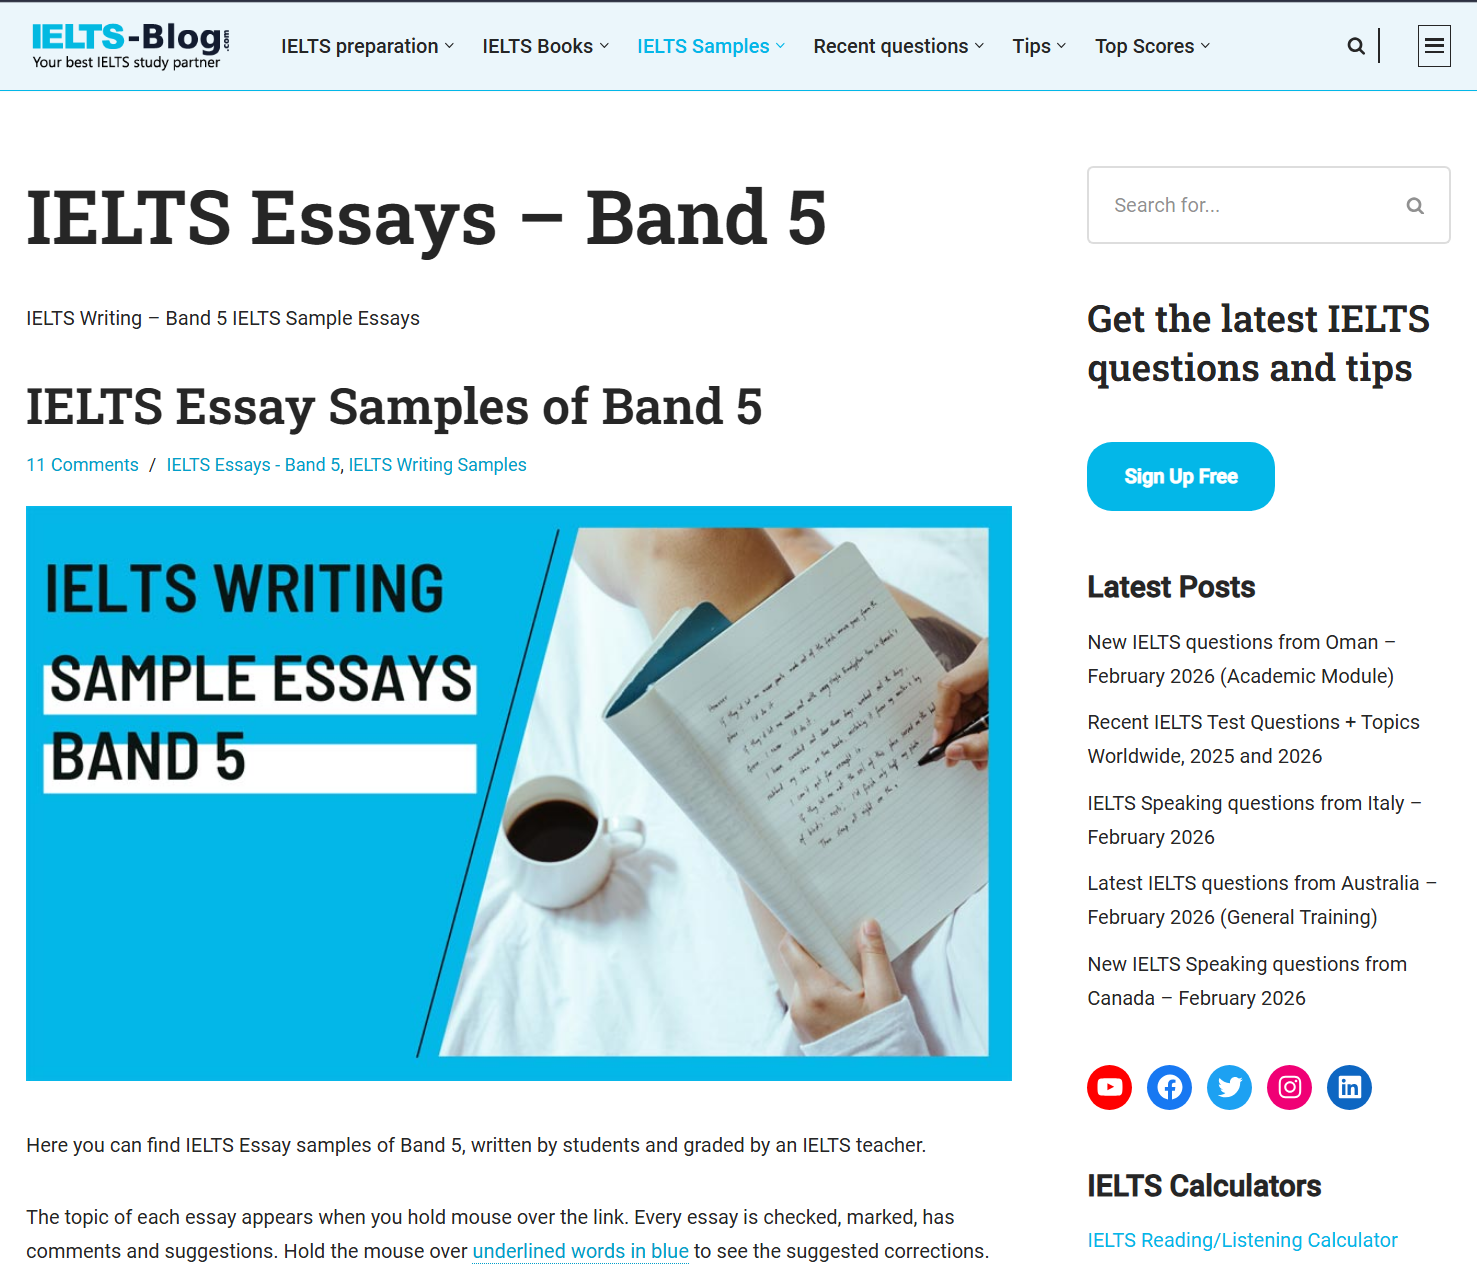
\includegraphics[width=0.92\linewidth]{graphics/writing/ielts_blog}
    \captionsetup{skip=5pt}
    \caption{Trang web IELTS Blog bổ sung thêm các bài viết và nhận xét từ môi trường ôn luyện thực tế}
    \label{fig:data-source-web}
\end{figure}

\subsubsection{Quy trình crawl và tiền xử lý dữ liệu}
Sau khi thu thập, dữ liệu được đưa về cùng một schema chuẩn gồm các trường \texttt{question\_content}, \texttt{essay\_content}, \texttt{task\_type}, \texttt{scores} và \texttt{feedback\_analysis}. Mỗi mẫu dữ liệu biểu diễn một cặp đầu vào -- đầu ra theo cấu trúc:
\begin{itemize}
    \item \textbf{Input:} đề bài IELTS Writing + bài viết của thí sinh.
    \item \textbf{Output:} điểm tổng, điểm thành phần và nhận xét chi tiết.
\end{itemize}

Trong bước làm sạch dữ liệu phục vụ huấn luyện, nhóm ưu tiên giữ lại các mẫu có thông tin điểm số đầy đủ và phần \texttt{feedback\_analysis} không rỗng, nhờ đó bảo đảm chất lượng nhãn đầu vào cho mô hình. Thu được data set gồm \textbf{7614} bản ghi, có \textbf{7610} mẫu chứa \textit{overall score} và \textbf{6919} mẫu có đủ cả 5 thành phần điểm. 

Để phù hợp với kiểu huấn luyện hội thoại, mỗi mẫu được chuyển thành ba message:
\begin{itemize}
    \item \textbf{System prompt:} định nghĩa vai trò mô hình là ``IELTS Academic Writing Tutor'', mô tả tiêu chí chấm điểm và yêu cầu phản hồi.
    \item \textbf{User message:} chứa đề bài và bài viết cần chấm.
    \item \textbf{Assistant message:} chứa đáp án mục tiêu theo format thống nhất gồm phần điểm số và phần feedback.
\end{itemize}

Sau đó, toàn bộ message được ghép bằng \texttt{tokenizer.apply\_chat\_template(...)} để tạo chuỗi huấn luyện đầu vào cho \texttt{SFTTrainer}.

\subsubsection{Đặc trưng của tập dữ liệu}
Kết quả phân tích dữ liệu cho thấy tập dữ liệu có một số đặc điểm chính như sau:
\begin{itemize}
    \item Trong tập phân tích mở rộng gồm 7614 bản ghi, có \textbf{7610} mẫu có overall score và \textbf{6919} mẫu có đủ cả 5 thành phần điểm.
    \item Phân bố \texttt{task\_type} lệch về \texttt{task\_2}: \textbf{6226} mẫu Task 2 (81.8\%) và \textbf{1388} mẫu Task 1 (18.2\%).
    \item Overall band score có giá trị trung bình \textbf{6.17}, trung vị \textbf{6.0}, độ lệch chuẩn \textbf{1.71}; các band phổ biến nhất là 7.5, 5.5, 6.0, 8.0 và 7.0.
    \item Độ dài bài viết trung bình dao động khoảng \textbf{257--294 từ} tùy nguồn dữ liệu; tương quan Pearson giữa độ dài bài viết và overall band score là \textbf{0.205}, cho thấy độ dài chỉ có tương quan dương yếu với chất lượng bài viết.
    \item Sau khi định dạng thành prompt huấn luyện, độ dài mẫu có mean khoảng \textbf{1028 tokens}, median \textbf{1024 tokens}, max \textbf{2845 tokens}, P99 khoảng \textbf{1412 tokens}. Với \texttt{MAX\_SEQ\_LENGTH = 4096}, không có mẫu nào bị cắt ngữ cảnh.
\end{itemize}

\begin{figure}[H]
    \centering
    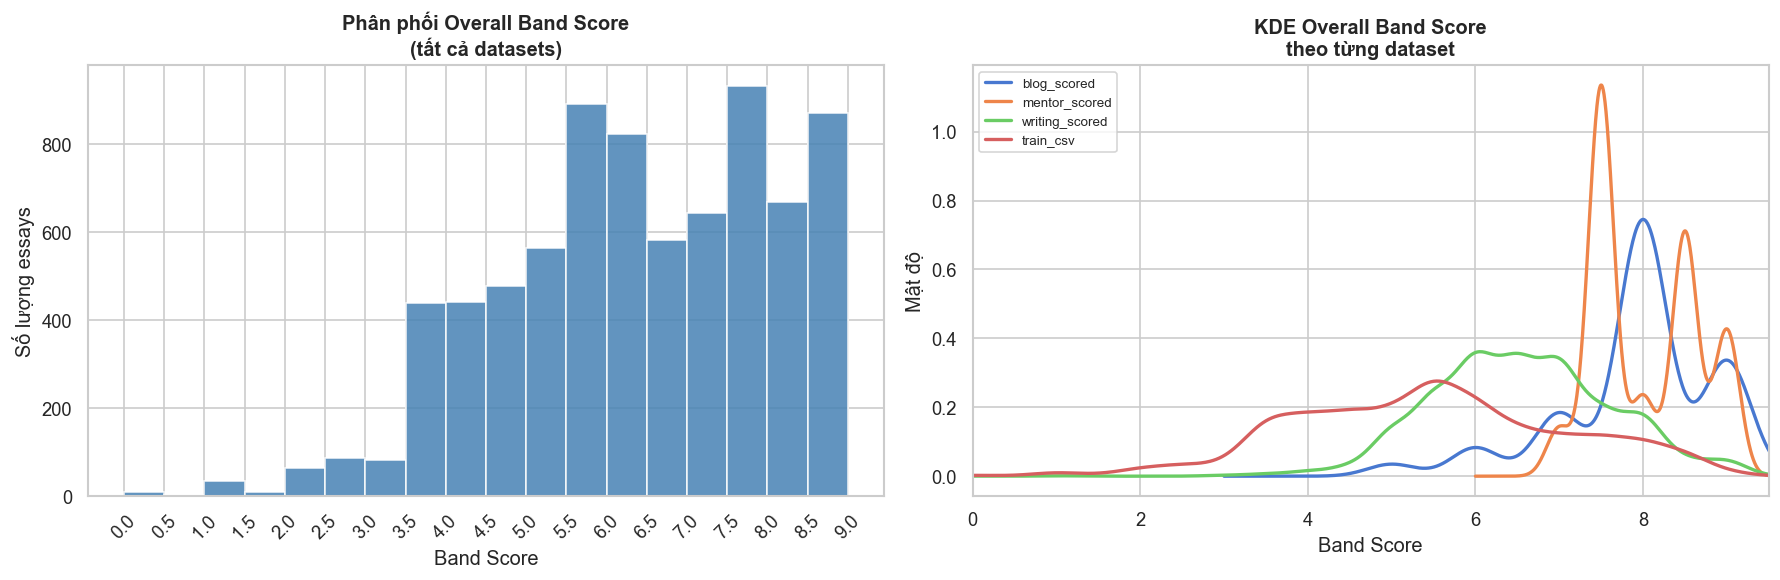
\includegraphics[width=0.9\linewidth]{graphics/writing/phan_phoi_data_set}
    \captionsetup{skip=5pt}
    \caption{Phân phối Overall Band Score}
    \label{fig:data-char-placeholder-1}
\end{figure}

\begin{figure}[H]
    \centering
    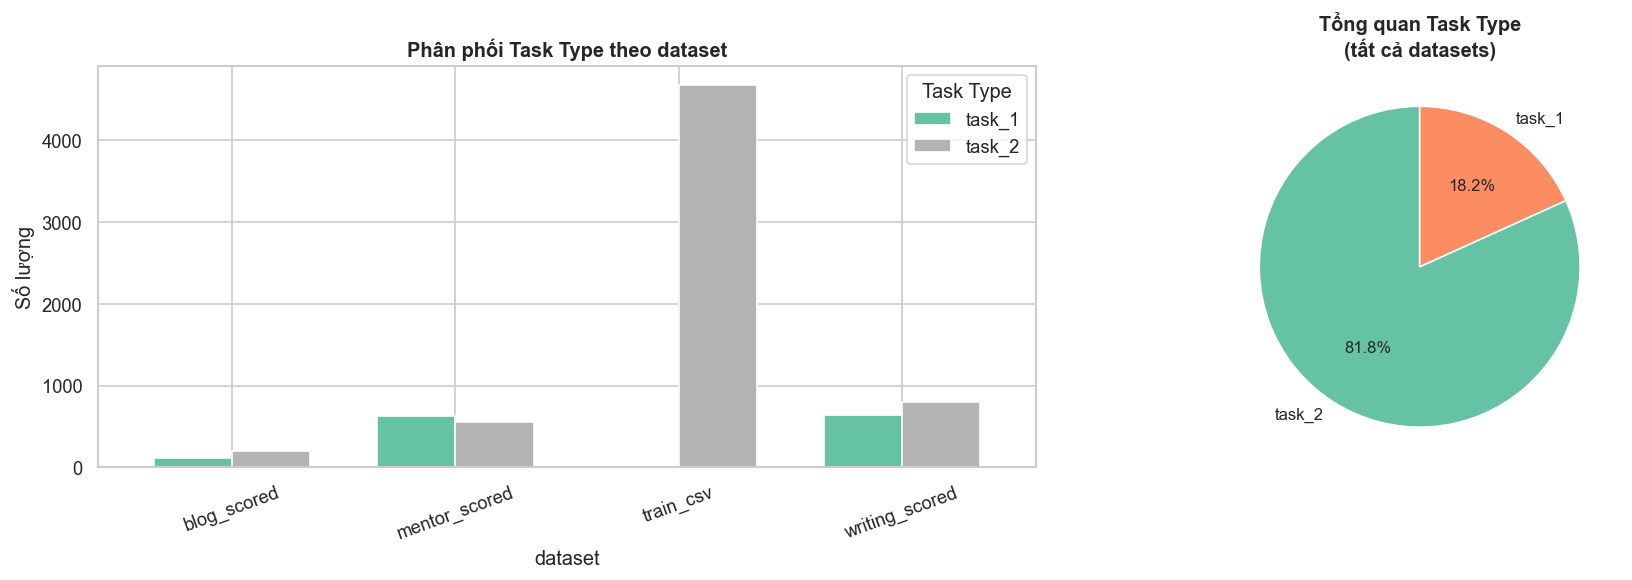
\includegraphics[width=0.9\linewidth]{graphics/writing/phan_phoi_task_type}
    \captionsetup{skip=5pt}
    \caption{Phân phối Task Type}
    \label{fig:data-char-placeholder-2}
\end{figure}

Tuy vậy, dữ liệu vẫn tồn tại một số hạn chế. Thứ nhất, phân bố task không cân bằng, nghiêng mạnh về Task 2. Thứ hai, chất lượng nhãn phụ thuộc vào nguồn công khai và các bài chấm sẵn, nên mức độ nhất quán giữa các nguồn có thể chưa hoàn toàn đồng nhất.

\subsection{Huấn luyện mô hình Phi-3 cho bài toán Writing}

\subsubsection{Lý do lựa chọn Phi-3}
Nhóm chọn \textbf{Phi-3-mini-4k-instruct} vì đây là mô hình có quy mô khoảng \textbf{3.8B tham số}, phù hợp với giới hạn tài nguyên của môi trường Kaggle nhưng vẫn đủ năng lực xử lý prompt dài và sinh phản hồi tự nhiên. Mô hình hỗ trợ ngữ cảnh 4k tokens, đủ cho cấu trúc đầu vào gồm đề bài, bài viết và chỉ dẫn chấm điểm. Ngoài ra, việc kết hợp phiên bản 4-bit với LoRA giúp giảm đáng kể chi phí bộ nhớ mà vẫn giữ được khả năng thích nghi cho tác vụ chuyên biệt.

\subsubsection{Chiến lược huấn luyện}
Nhóm áp dụng chiến lược \textbf{QLoRA}, tức fine-tune mô hình lượng tử hóa 4-bit bằng các adapter LoRA. Cấu hình chính gồm:
\begin{itemize}
    \item Base model: \texttt{unsloth/Phi-3-mini-4k-instruct-bnb-4bit}
    \item \texttt{max\_seq\_length = 4096}
    \item LoRA rank \texttt{r = 16}, \texttt{lora\_alpha = 16}, \texttt{lora\_dropout = 0}
    \item Các lớp được gắn adapter: \texttt{q\_proj}, \texttt{k\_proj}, \texttt{v\_proj}, \texttt{o\_proj}, \texttt{gate\_proj}, \texttt{up\_proj}, \texttt{down\_proj}
\end{itemize}

Với cấu hình này, số tham số cần huấn luyện chỉ khoảng \textbf{29.9M} trên tổng số gần \textbf{2.0B} tham số đang hoạt động, tương đương khoảng \textbf{1.47\%}. Điều này giúp bài toán huấn luyện khả thi trên GPU T4 mà không cần hạ đáng kể độ dài ngữ cảnh hoặc batch size.

\subsubsection{Quy trình thực nghiệm}
Pipeline thực nghiệm được triển khai trên Kaggle theo các bước:
\begin{enumerate}
    \item Nạp và làm sạch dữ liệu từ các file scored.
    \item Xây dựng prompt template theo định dạng chat.
    \item Phân tích token length để lựa chọn context length phù hợp.
    \item Chia dữ liệu theo chiến lược \textit{stratified split} dựa trên overall band score với tỉ lệ \textbf{90\% train} và \textbf{10\% eval}.
    \item Huấn luyện mô hình bằng \texttt{SFTTrainer} của TRL kết hợp thư viện Unsloth.
    \item Theo dõi \texttt{train\_loss}, \texttt{eval\_loss} theo từng bước và chọn checkpoint tốt nhất.
\end{enumerate}

Sau khi chia dữ liệu, tập train có \textbf{4775 mẫu} và tập eval có \textbf{531 mẫu}. Các siêu tham số huấn luyện chính gồm:
\begin{itemize}
    \item \texttt{per\_device\_train\_batch\_size = 2}
    \item \texttt{gradient\_accumulation\_steps = 4} (batch hiệu dụng bằng 8)
    \item \texttt{learning\_rate = 2e-4}
    \item \texttt{lr\_scheduler\_type = cosine}
    \item \texttt{warmup\_ratio = 0.05}
    \item \texttt{num\_train\_epochs = 3}
    \item \texttt{optim = adamw\_8bit}
    \item \texttt{weight\_decay = 0.01}
    \item \texttt{max\_grad\_norm = 0.3}
    \item \texttt{seed = 42}
\end{itemize}

\subsubsection{Kết quả huấn luyện}
Thí nghiệm được chạy trên môi trường Kaggle GPU với \textbf{Tesla T4}, trong notebook có hỗ trợ chạy trên cấu hình \textbf{T4x2} bằng \texttt{device\_map="auto"}. Kết quả huấn luyện chính như sau:
\begin{itemize}
    \item Số epoch: \textbf{3}
    \item Tổng số bước huấn luyện: khoảng \textbf{1791 steps}
    \item Thời gian huấn luyện: khoảng \textbf{25545 giây} (xấp xỉ 7 giờ)
    \item Final train loss: khoảng \textbf{0.8757}
    \item Peak GPU memory quan sát được: khoảng \textbf{3.7 GB}
\end{itemize}

Mô hình sau huấn luyện cho đầu ra đúng cấu trúc mong muốn, gồm mục \texttt{IELTS Writing Evaluation}, phần \texttt{Scores} với 5 thang điểm và phần \texttt{Detailed Feedback}. Điều này cho thấy mô hình đã học được cả khuôn dạng phản hồi lẫn nhiệm vụ chấm điểm trên dữ liệu chuyên biệt.

\subsection{Triển khai mô hình sau huấn luyện}

\subsubsection{Kiến trúc triển khai}
Sau khi huấn luyện xong, mô hình được lưu tại thư mục làm việc trên Kaggle dưới dạng adapter LoRA, tokenizer, chat template và metadata để phục vụ tái lập thí nghiệm. Đồng thời, nhóm chuyển đổi mô hình sang định dạng 	\textbf{GGUF} và đẩy lên \textbf{Hugging Face} nhằm quản lý version một cách nhất quán, thuận tiện cho việc theo dõi các lần cập nhật mô hình, tái sử dụng trong suy luận và triển khai ở các môi trường khác nhau. Ở giai đoạn triển khai, mô hình được đưa lên \textbf{Hugging Face Inference Endpoint} để tạo một endpoint suy luận ổn định cho mô-đun Writing. Trên hệ thống ứng dụng, nhóm xây dựng một \textbf{Writing service} làm lớp trung gian: service này nhận request từ backend, gọi tới Hugging Face endpoint để lấy kết quả suy luận, sau đó đóng gói dữ liệu phản hồi và chuyển tiếp về hệ thống chính.

Để tách biệt xử lý đồng bộ và bất đồng bộ, Writing service giao tiếp với backend chính thông qua \textbf{RabbitMQ}. Cách tổ chức này giúp backend không phải gọi trực tiếp tới mô hình, đồng thời thuận tiện hơn cho việc mở rộng, giám sát và xử lý retry khi có lỗi trong quá trình sinh kết quả.

\subsubsection{Pipeline suy luận}
Pipeline suy luận trong hệ thống có thể mô tả như sau:
\begin{enumerate}
    \item Người dùng nhập đề bài và bài viết ở giao diện Writing.
    \item Backend chính tiếp nhận request và đẩy thông điệp sang hàng đợi RabbitMQ.
    \item Writing service lấy dữ liệu từ RabbitMQ, chuẩn hóa input theo đúng prompt template đã dùng trong quá trình huấn luyện.
    \item Writing service gọi tới Hugging Face Inference Endpoint chứa mô hình Phi-3 đã fine-tune.
    \item Endpoint trả về điểm tổng, điểm thành phần và phản hồi chi tiết cho bài viết.
    \item Writing service đóng gói kết quả và gửi lại qua RabbitMQ để backend chính nhận và trả về giao diện người dùng.
\end{enumerate}

\subsubsection{Các vấn đề triển khai thực tế}
Về mặt triển khai, bài toán Writing đặt ra một số yêu cầu thực tế. Thứ nhất là cần tối ưu độ trễ suy luận do đầu vào thường dài hơn các bài toán hỏi đáp ngắn. Thứ hai là cần bảo toàn đúng prompt format giữa giai đoạn train và infer; vì vậy chat template được lưu kèm mô hình và tái sử dụng tại Writing service. Thứ ba là cần một cơ chế giao tiếp ổn định giữa mô-đun AI và backend chính; RabbitMQ được sử dụng để tách tải, hỗ trợ xử lý bất đồng bộ và giảm ghép nối trực tiếp giữa các thành phần hệ thống.

\subsection{Đánh giá và ý nghĩa của mô-đun Writing}
Để đánh giá chất lượng mô hình, nhóm xây dựng notebook nhằm so sánh mô hình đã fine-tune với \textbf{GPT o4-mini}. Việc đánh giá được thực hiện dựa trên các \textbf{metric phản ánh chất lượng dự đoán} như MAE, RMSE, hệ số tương quan Pearson, tỉ lệ dự đoán nằm trong ngưỡng sai số 0.5 và 1.0 band, cùng độ lệch trung bình so với điểm tham chiếu.

Các metric này được lựa chọn vì phù hợp trực tiếp với bản chất của bài toán chấm điểm IELTS Writing. Trước hết, đầu ra của mô hình là \textbf{điểm số liên tục theo thang band}, nên cần các metric đo \textbf{mức sai lệch định lượng} giữa điểm dự đoán và điểm tham chiếu, thay vì chỉ đánh giá đúng hoặc sai tuyệt đối như trong bài toán phân loại. Trong đó, \textbf{MAE} cho biết trung bình mô hình lệch bao nhiêu band so với điểm thật, là một chỉ số dễ diễn giải trong ngữ cảnh chấm điểm. Ví dụ, MAE xấp xỉ 0.5 có thể hiểu là trung bình mỗi bài viết bị lệch nửa band, đây là mức sai số có ý nghĩa thực tế trong IELTS.

Bên cạnh đó, \textbf{RMSE} được sử dụng để nhấn mạnh tác động của các dự đoán sai lệch lớn. Trong bài toán chấm Writing, một số trường hợp chấm lệch quá xa, chẳng hạn chênh 1.5 hoặc 2.0 band, có thể gây ảnh hưởng đáng kể đến trải nghiệm học tập và độ tin cậy của hệ thống. Do RMSE phạt mạnh hơn các sai số lớn, metric này giúp phản ánh mức độ ổn định của mô hình và khả năng hạn chế các dự đoán bất thường.

\textbf{Hệ số tương quan Pearson} được đưa vào để đánh giá xem mô hình có bám theo xu hướng phân bố điểm thực tế hay không. Trong thực tế, một mô hình tốt không chỉ cần dự đoán gần điểm thật ở trung bình, mà còn cần giữ được quan hệ thứ tự tương đối giữa các bài viết yếu, trung bình và tốt. Nếu hệ số tương quan cao, điều đó cho thấy khi chất lượng bài viết tăng hoặc giảm, điểm dự đoán của mô hình cũng biến thiên cùng chiều một cách hợp lý.

Ngoài các metric sai số tổng quát, nhóm sử dụng thêm \textbf{tỉ lệ dự đoán nằm trong ngưỡng sai số 0.5 band và 1.0 band} vì đây là cách đánh giá rất phù hợp với thang điểm IELTS. Trong bối cảnh chấm bài Writing, chênh lệch 0.5 band thường được xem là một mức sai số nhỏ và có thể chấp nhận được trong nhiều tình huống hỗ trợ học tập, trong khi chênh lệch 1.0 band là ngưỡng rộng hơn để đánh giá khả năng bám sát tổng thể. Hai metric này vì thế giúp chuyển kết quả từ dạng số học thuần túy sang cách hiểu gần hơn với thực tế sử dụng của hệ thống.

Cuối cùng, \textbf{độ lệch trung bình (bias)} được sử dụng để kiểm tra xu hướng chấm thiên lệch của mô hình. Với bài toán IELTS Writing, một mô hình có thể đạt sai số trung bình tương đối thấp nhưng vẫn có xu hướng \textit{over-predict} hoặc \textit{under-predict} một cách hệ thống. Việc theo dõi bias giúp nhận diện xem mô hình có xu hướng chấm cao hơn hoặc thấp hơn điểm tham chiếu hay không, từ đó đánh giá được tính công bằng và độ tin cậy của hệ thống khi triển khai thực tế.

Nhìn chung, tập hợp các metric trên được lựa chọn nhằm phản ánh đồng thời nhiều khía cạnh của bài toán chấm điểm IELTS Writing: độ lệch trung bình, mức độ nhạy với sai số lớn, khả năng bám theo xu hướng điểm thực tế, mức sai số chấp nhận được theo thang band, và xu hướng thiên lệch khi chấm điểm. Cách đánh giá này phù hợp hơn với đặc thù của bài toán so với việc chỉ sử dụng một metric đơn lẻ.


Trên số mẫu thu được, mô hình \textbf{Phi-3 SFT} đạt:
\begin{itemize}
    \item \textbf{MAE = 0.976}
    \item \textbf{RMSE = 1.332}
    \item \textbf{Pearson r = 0.638}
    \item \textbf{Within 0.5 band = 51.0\%}
    \item \textbf{Within 1.0 band = 71.0\%}
    \item \textbf{Bias = +0.049}
\end{itemize}

Trong khi đó, \textbf{GPT o4-mini} trên phần dữ liệu đánh giá được đạt:
\begin{itemize}
    \item \textbf{MAE = 1.205}
    \item \textbf{RMSE = 1.487}
    \item \textbf{Pearson r = 0.566}
    \item \textbf{Within 0.5 band = 35.8\%}
    \item \textbf{Within 1.0 band = 56.0\%}
    \item \textbf{Bias = -0.684}
\end{itemize}

\begin{figure}[H]
    \centering
    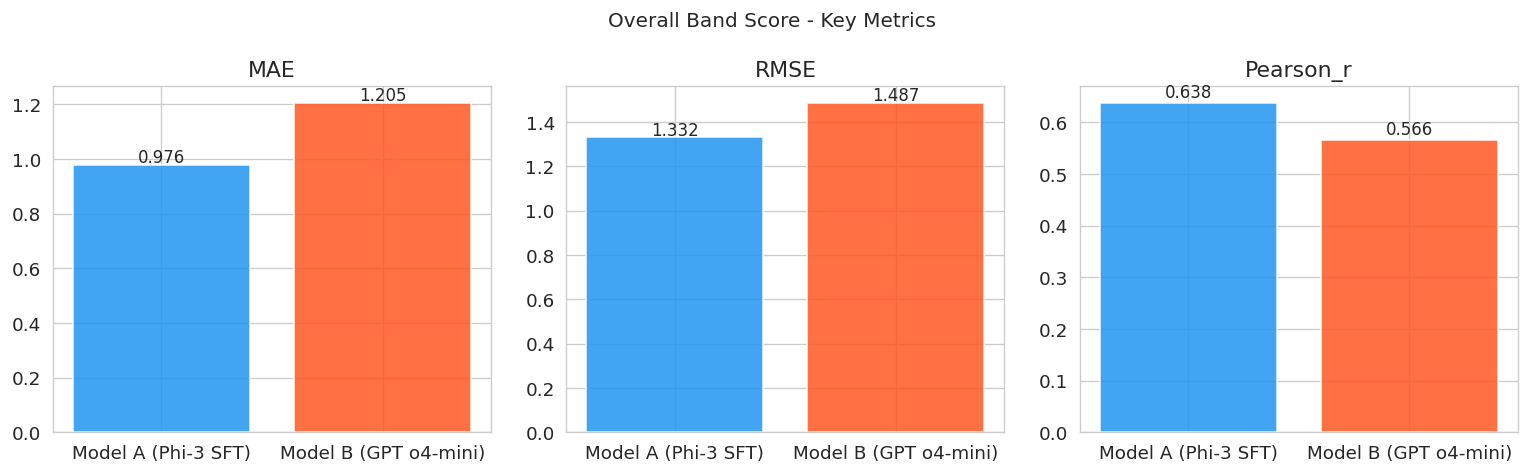
\includegraphics[width=0.88\linewidth]{graphics/writing/evaluate_band_score.png}
    \captionsetup{skip=5pt}
    \caption{So sánh kết quả đánh giá Writing giữa mô hình Phi-3 SFT và GPT o4-mini theo điểm dự đoán}
\end{figure}

\begin{figure}[H]
    \centering
    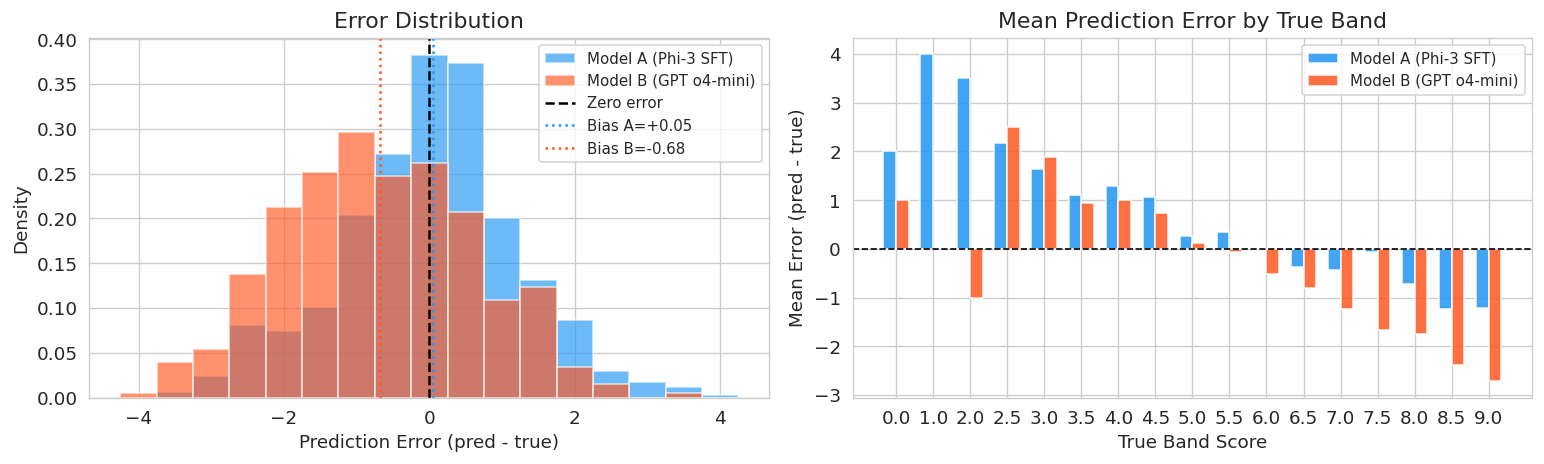
\includegraphics[width=0.88\linewidth]{graphics/writing/evaluate_error.png}
    \captionsetup{skip=5pt}
    \caption{So sánh sai số đánh giá Writing của mô hình Phi-3 SFT và GPT o4-mini}
\end{figure}

Các metric trên cho thấy mô hình \textbf{Phi-3 SFT} cho kết quả tốt hơn \textbf{GPT o4-mini} trong thí nghiệm hiện tại ở nhiều khía cạnh: sai số tuyệt đối trung bình thấp hơn, tương quan với điểm thật cao hơn và tỉ lệ dự đoán nằm trong ngưỡng sai số 0.5 hoặc 1.0 band cũng tốt hơn. Điều này cho thấy việc fine-tune trên dữ liệu IELTS Writing chuyên biệt giúp mô hình bám sát tiêu chí chấm điểm của bài toán hơn so với việc sử dụng trực tiếp một mô hình tổng quát.

Bên cạnh đó, hướng triển khai mô hình nội bộ thông qua Hugging Face endpoint và Writing service còn mang lại ý nghĩa thực tế cho hệ thống: giảm phụ thuộc vào API chấm ngoài, chủ động hơn trong kiểm soát phiên bản mô hình, và tạo nền tảng để mở rộng sang các tác vụ khác như sinh phản hồi cá nhân hóa hoặc gợi ý sửa bài theo từng tiêu chí.

Tổng thể, mô-đun Writing là minh chứng rằng việc xây dựng một mô hình chuyên biệt cho miền dữ liệu IELTS Writing là khả thi trong phạm vi đồ án. Quá trình phân tích dữ liệu, chuẩn hóa đầu vào, huấn luyện bằng QLoRA và chuẩn bị pipeline triển khai đã tạo ra một nền tảng đủ vững để tiếp tục cải tiến thành tính năng chấm và phản hồi bài viết thực tế trong hệ thống luyện thi tiếng Anh.


\section{Kết luận chương}
Chương này cho thấy AI trong hệ thống không chỉ được dùng như một thành phần bổ sung, mà đóng vai trò trung tâm trong việc thiết kế trải nghiệm học tập. Với kỹ năng Speaking, Lingriser là minh họa rõ nét cho cách kết hợp hội thoại AI, phiên âm, tổng hợp tiếng nói, theo dõi tiến trình và điều phối sư phạm trong một nền tảng thống nhất. Với kỹ năng Writing, hệ thống định hướng khai thác AI để phân tích bài viết và chấm điểm theo tiêu chí band score.

Việc tách riêng hai hướng Speaking và Writing giúp làm rõ đặc thù dữ liệu, mục tiêu đánh giá và cách tích hợp AI cho từng kỹ năng. Đồng thời, chương này cũng tạo cơ sở để các phần sau có thể tiếp tục đánh giá sâu hơn về hiệu quả, khả năng mở rộng và giá trị thực tiễn của các mô-đun AI trong toàn bộ hệ thống.